\documentclass[11pt, oneside]{article}   	% use "amsart" instead of "article" for AMSLaTeX format
\usepackage{geometry}                		% See geometry.pdf to learn the layout options. There are lots.
\geometry{letterpaper}                   		% ... or a4paper or a5paper or ... 
%\geometry{landscape}                		% Activate for for rotated page geometry
%\usepackage[parfill]{parskip}    		% Activate to begin paragraphs with an empty line rather than an indent
\usepackage{graphicx}				% Use pdf, png, jpg, or eps§ with pdflatex; use eps in DVI mode
								% TeX will automatically convert eps --> pdf in pdflatex		
\usepackage{amssymb}
\usepackage{amsmath}
\usepackage{parskip}
\usepackage{color}
\usepackage{hyperref}

\title{Complex function theory}
%\author{The Author}
%\section{}
%\subsection*{}
\date{}							% Activate to display a given date or no date

\graphicspath{{/Users/telliott_admin/Dropbox/Tex/png/}}
% \begin{center} 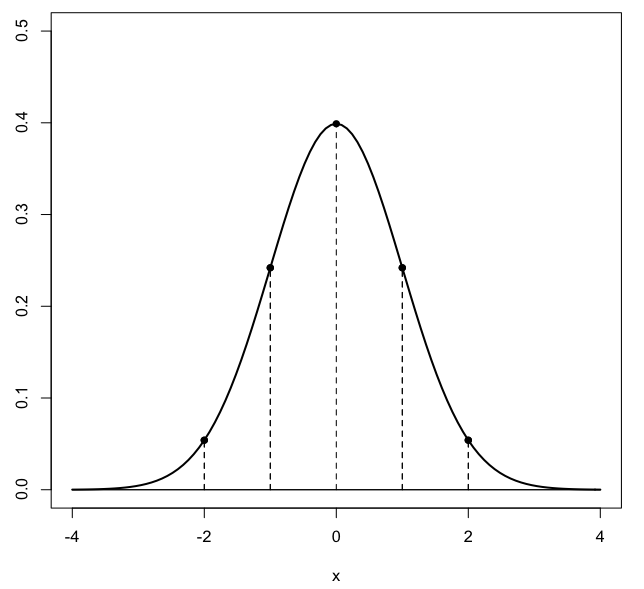
\includegraphics [scale=0.4] {gauss3.png} \end{center}
\begin{document}
\maketitle
\Large

\section{Arithmetic}
Complex numbers arose in the context of finding solutions to certain polynomials, for example:
\[ x^2 + 1 = 0 \]
and
\[ x^2 + x + 1 = 0 \]
For the first equation, it is easy to see that there is no solution among the real numbers since $x^2$ is always positive or zero.  So adding $1 + x^2$ cannot bring the sum back to zero.

Visualizing the same function geometrically, this is just the simple parabola $y=x^2$ shifted up by one unit, moving its vertex from $(0,0)$ to $(0,1)$.  Plotting shows that the graphs of both functions never cross the $x$-axis---there are no values that lie on the curve and also on the line $y=0$.

The ingenious solution to this problem is to invent a new kind of number
\[ i = \sqrt{-1} \ , \ \ \ i^2 = -1 \]
Once we accept that $i = \sqrt{-1}$
then
\[ (x + i)(x - i) = x^2 - i^2 \]
\[ = x^2 - (-1) = x^2 + 1 \]
so $\pm \ i$ are both solutions to the above equation.

For the second one
\[ x^2 + x + 1 = 0 \]
we can plot it, or we can factor it, or recall the quadratic formula for solutions to
\[ ax^2 + bx + c = 0 \]
for real constants $a$, $b$ and $c$.  The formula is
\[ \frac{-b \pm \sqrt{b^2 - 4ac}}{2a} \]
When $4ac > b^2$, then the solutions to the quadratic formula involve the square root of a negative number.  Here the formula gives
\[ \frac{-1 \pm \sqrt{-3}}{2} \]
Check the positive root:
\[ x^2 = (\frac{-1 + \sqrt{-3}}{2})^2 \]
\[ = \frac{1}{4} - \frac{\sqrt{-3}}{2} - \frac{3}{4} \]
Adding this to $x+1$ we obtain
\[  \frac{1}{4} - \frac{\sqrt{-3}}{2} - \frac{3}{4}  + \frac{-1 + \sqrt{-3}}{2} + 1 \]
the terms with $\sqrt{-3}$ cancel, giving
\[ = \frac{1}{4} - \frac{3}{4}  - \frac{1}{2} + 1 = 0 \]

In fact, now that we have $i$ available, any square root like $\sqrt{-(a^2)}$, where $a$ is a real number, can be factored as $\sqrt{-1} \ \sqrt{a^2} = ia$.

Note that the converse is not necessarily true.  Consider
\[ i^2 = \sqrt{-1} \cdot \sqrt{-1} \stackrel{?}{=} \sqrt{(-1)\cdot (-1)} = \sqrt{1} \]

Now, $\sqrt{1}$ has two solutions or roots (since $-1 \times -1$ and $1 \times 1$ are both equal to $1$), but we choose the positive root when thinking about $\sqrt{x}$ as a \emph{function}.  However, $i^2$ was defined to be equal to $-1$, not $1$.  What's the deal?

The problem is that the equality with a question mark is not valid
\[ \sqrt{-1} \cdot \sqrt{-1} \ne \sqrt{(-1)\cdot (-1)} \]
which explains why this "proof" is erroneous.

Expressions that involve the square root of a negative real number, like $\sqrt{-1} = i$ and $\sqrt{-3} = \sqrt{3}\ i$, are called imaginary (or \emph{purely} imaginary).  

Numbers that contain both a real and an imaginary part, like $1 + i$, are termed complex numbers, and imaginary numbers are considered to be complex numbers with the real part equal to $0$.

We say that the set of complex numbers $\mathbb{C}$ includes the real numbers:
\[ \mathbb{R} \subset \mathbb{C} \]

We write complex numbers $z$ as combinations like
\[ z = a + ib \]
 where $a$ and $b$ are both real numbers.  $a$ is the real part, and $b$ the imaginary part of the complex number $z$.

Some useful identities involving $i$ include
\[ i^2 = -1 \ , \ \ \  i = -\frac{1}{i} \ , \ \ \  -i = \frac{1}{i} \]

It turns out that for much of what is done with complex numbers the fact that $i$ equals $\sqrt{-1}$ is not even relevant.

Instead, we simply think of \emph{ordered pairs} of real numbers $(a,b)$ and the $i$ notation is a bookkeeping device, a marker to remind us that when we multiply two complex numbers
\[ (a + ib) (c + id) = ac + a \cdot id + ib \cdot c + ib \cdot id \]
the last term gets a minus sign:
\[ ib \cdot id = -bd \]
The result of multiplying $ib \cdot id$ is a real number with the sign flipped, while a real number $a$ times an imaginary number $id$ is equal to $iad$ and
\[ (a + ib) (c + id) = ac -bd + i(ad + bc) \]

Note carefully that if we consider two complex numbers $z_1 = a + ib$ and $z_2 = c + id$, then 
\[ z_1 = z_2 \iff a = c \text{ and } b = d \]
Two complex numbers $z_1$ and $z_2$ are equal \emph{if and only if} both the real and the imaginary parts are equal.

Another way to keep track of the same information is in matrix form, namely:
\[
z = \begin{bmatrix}
a & -b \\
b &  \ \ a
\end{bmatrix}
\]
Such matrices can be added and multiplied in the normal way and give the desired results for complex numbers.  Thus:
\[
\begin{bmatrix}
a & -b \\
b &  \ \ a
\end{bmatrix} \times
\begin{bmatrix}
c & -d \\
d &  \ \ c
\end{bmatrix} =
\begin{bmatrix}
ac + bd & -ad - bc \\
ad + bc &  \ \ ac + bd
\end{bmatrix} 
=
\begin{bmatrix}
 u & -v \\
v &  \ \ u
\end{bmatrix}
\]
\subsection*{Argand plane}
Yet another way to think about complex numbers is to use the complex plane (the Argand plane), where points are plotted with the real part along the horizontal axis and the imaginary part along the vertical axis.

This figure is from Brown \& Churchill.
\begin{center} 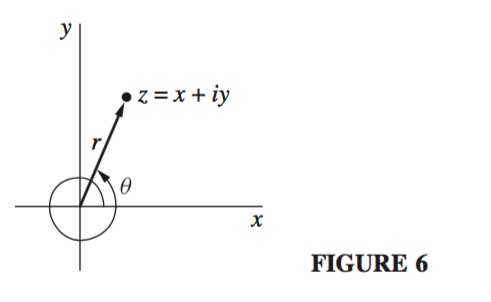
\includegraphics [scale=0.6] {Brown6.png} \end{center}

Looking at the graph, the distance of any point from the origin is denoted by $r$, and $\theta$ is the angle the ray makes with the positive $x$-axis in a CCW direction.  This should be familiar from standard polar coordinates.

Switching notation to
\[ z = x + iy \]
To plot the complex number $z$ we go out $x$ units along the real (horizontal) axis and then up $y$ units along the imaginary (vertical) axis.

The statement that $\mathbb{R} \subset \mathbb{C}$ is equivalent to the observation that the Argand plane contains the horizontal axis.  Real numbers have the form $z = x + i \cdot 0 = x$.

More generally, though
\[ x = r \cos \theta \]
\[ y = r \sin \theta \]
and
\[ x + iy = r \cos \theta + ir \sin \theta\]
\[ = r(\cos \theta + i \sin \theta) \]
\[ = re^{i\theta} \]
where the last part makes use of Euler's famous equation.  $r$ is called the \textbf{modulus} and $\theta$ is called the \textbf{argument} or \textbf{phase}.

Notice that in the figure above the argument $\theta$ is actually $\theta + 2 \pi$.  All multiples $k \cdot 2 \pi$ for $k \in 0, \pm 1, \pm 2 \dots$ are valid.

Calculations are often easier using one form rather than another.  Addition is simpler with $a + ib$ (the Cartesian format) since
\[ (a + ib) + (c + id) = (a+c) + i (b + d) \]
 while multiplication is more straightforward with the polar format.  Matrices work fine for both addition and multiplication.
 
Here is multiplication in polar coordinates
\[ r e^{i\theta} \ \rho e^{i\phi} = r \rho \ e^{i (\theta + \phi)} \]
We multiply the distances and add the angles.  Here is the square function:
\[ (r e^{i\theta})^2 = r^2 e^{i2\theta} \]

Multiplication of $z_1 = r_1 e^{i\theta_1}$ by $z_2 = r_2 e^{i\theta_2}$ stretches $r_1$ (the length of $z_1$) by the factor $r_2$ (the length of $z_2$), and rotates $z_1$ by adding a phase shift of $\theta_2$ to the original angle $\theta_1$.
\begin{center} 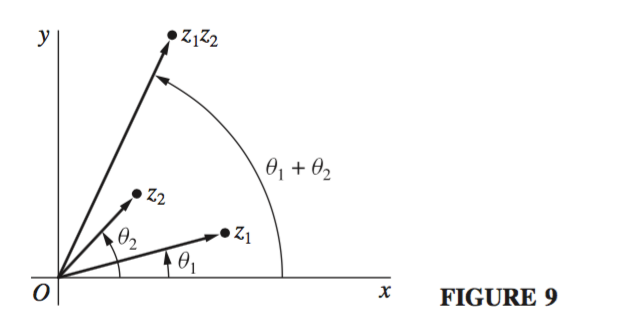
\includegraphics [scale=0.6] {Brown9.png} \end{center}

\section{Conjugate}
Consider the complex number:
\[ z = x + iy \]
The complex conjugate of $z$ (called $z*$ or $\bar{z}$) is given by:
\[ z* = x - iy \]
The real part of $z*$ is the same as the real part of $z$, while the imaginary part has the signs switched.

The \emph{length} of $z$ squared is equal to $z$ multiplied by its complex conjugate
\[ zz* = (x + iy) (x - iy) \]
\[ =  x^2 - ixy + ixy -i^2y^2 \]
\[ = x^2 + y^2 \]
\[ = r^2 \cos^2 \theta + r^2 \sin^2 \theta \]
\[ = r^2   \]
Again, $r$ is the length of the ray from the origin to $z$ as plotted in the complex plane.
\[ r^2 = zz* \]
\[ r = \sqrt{zz*} \]
The point corresponding to $z*$ in the complex plane has the same overall distance from the origin and the same $x$-component as $z$, but the sign change on $y$ means that $z*$ is reflected across the $x$-axis from $z$.
\begin{center} 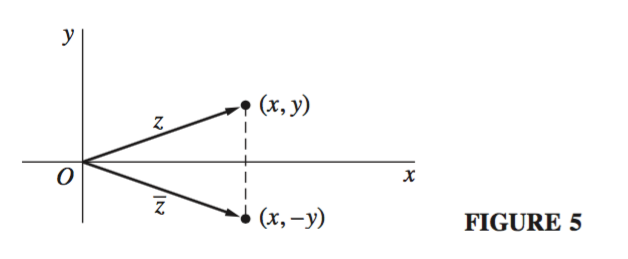
\includegraphics [scale=0.6] {Brown5.png} \end{center}

In polar coordinates, if $z = re^{i \theta}$ then $z* = re^{i (- \theta)} = re^{-i\theta}$.  So
\[ zz* = re^{i \theta} \ re^{i - \theta} = r^2 e^0 = r^2 \]
Multiplication of $z$ by $z*$ makes the product entirely real.  

If we consider addition rather than multiplication of the complex conjugate we observe that it also gives an entirely real result:
\[ z + z* = x + iy + x - iy = 2x \]
while subtraction gives an entirely imaginary result:
\[ z - z* = x + iy - x + iy = i2y \]

Another result (that we state without proof) is that if we have an expression involving several complex numbers:
\[ w = f(z_1, z_2 \dots) \]
we can obtain the complex conjugate of the whole thing by substituting the complex conjugate of each component:
\[ w* = f(z_1*, z_2* \dots) \]
An example might be
\[ z*z* = (x - iy)(x - iy) \]
\[ = x^2 - y^2 - i2xy \]
\[ = (zz)* \]
since
\[ zz = (x + iy)(x + iy) \]
\[ = x^2 - y^2 + i2xy \]
which has just flipped the sign on the imaginary part from the previous result, forming its complex conjugate.

\section{Differentiate}
This section contains a general discussion of differentiation of complex functions, which gives us a first glimpse of the important Cauchy-Riemann conditions and justifies the formula
\[ f'(z) = u_x + i v_x \]

As an example of its use, in the next section we will see that the complex exponential is
\[ f(z) = e^z = e^x e^{iy} \]
\[ = e^x (\cos y + i \sin y) \]
and using the formula, it can be shown easily that the derivative is the same as the function itself, just as for the case of real numbers.

\subsection*{definition}
We define the derivative $f'(z)$ of a complex function $f(z)$ similarly to the derivative of a real function.  We say that:
\[ f'(z) = \lim_{w \rightarrow z} \ \frac{f(w) - f(z)}{w-z} \]
Alternatively
\[ f'(z) = \lim_{\Delta z \rightarrow 0} \ \frac{f(z + \Delta z) - f(z)}{\Delta z} \]

A crucial point is that the limit is over all possible ways of approaching $z$ in the Argand plane.  If the limit exists, the function $f$ is called differentiable and $f'(z)$ is the derivative.
Consider
\[ f(z) = u(x,y) + i v(x,y) \]
Then
\[ f'(z) = \frac{f(z + \Delta z) - f(z)}{\Delta z} \]
\[ = \frac{u(x + \Delta x, y + \Delta y) + i v (x + \Delta x, y + \Delta y) - u(x,y) - i v(x,y)}{\Delta x + i \Delta y} \]

\subsection*{fixed y}
Looking at the special path along the $x$-axis where $\Delta y = 0$ we obtain
\[ f'(z) = \frac{u(x + \Delta x, y) + i v (x + \Delta x, y) - u(x,y) - i v(x,y)}{\Delta x} \]
Rearrange the numerator
\[ = \frac{u(x + \Delta x, y) - u(x,y)}{\Delta x} + \frac{i v (x + \Delta x, y) - i v(x,y)}{\Delta x} \]
The first term is
\[ u_x = \frac{\partial u}{\partial x} \]
and the second term is 
\[ i v_x \]
Hence we conclude that
\[ f'(z) = u_x + i v_x \]

\subsection*{fixed x}
Now look at the special path along the $y$-axis where $\Delta x = 0$:
\[ f'(z) = \frac{u(x, y + \Delta y) + i v (x, y + \Delta y) - u(x,y) - i v(x,y)}{i \Delta y} \]
Rearrange the numerator
\[ = \frac{u(x, y + \Delta y) - u(x,y)}{i \Delta y} + \frac{i v (x, y + \Delta y) - i v(x,y)}{i \Delta y} \]
\[ = \frac{1}{i} u_y + v_y \]
Recall that $1/i = -i$
\[ f'(z) = v_y - i u_y \]

\subsection*{Putting it together}
We require that the limit be the same regardless of the direction of approach to $z$, so in particular, these two expressions for the difference quotient must be equal:
\[ f'(z) = u_x + i v_x = - i u_y + v_y \]
Both the real and the imaginary parts must be equal so
\[ u_x  = v_y \]
\[ u_y = - v_x \]
And, as we said at the beginning, in looking at various complex functions we can use this fact:
\[ f'(z) = u_x + i v_x \]
In other words
\[ \frac{df}{dz} = \frac{\partial f}{\partial x} \]
and since
\[ u_x + i v_x = v_y - i u_y \]
\[ \frac{df}{dz} = -i \frac{\partial f}{\partial y} \]

\subsection*{more}
When we get to integration in a later section we will find that we integrate complex functions as line integrals along a specified curve (perhaps a circle centered on the origin or on a point $z_0$).  This curve relates the values of $x$ and $y$ and allows us to parametrize either $y$ in terms of $x$ or more generally, both $x$ and $y$ in terms of a single real variable or parameter $t$.

When we have a function of such a variable like
\[ f(t) = u(t) + i v(t) \]
then the derivative is defined to be
\[ f'(t) = u'(t) + i v'(t) \]
where $u$ and $v$ are real-valued functions of a single real variable and so follow the standard rules from introductory calculus.  In particular if
\[ w(t) = z_0 f(t) \]
then
\[ w'(t) = z_0 f'(t) \]
We can show this by using a little algebra:
\[ \frac{d}{dt} \ z_0 f(t) = \ [ \ (x_0 + i y_0) (u + iv) \ ]' \]
\[ = \ [ \ (x_0 u - y_0 v) + i (y_0 u + x_0 v) \ ]' \]
\[ = (x_0 u - y_0 v)' + i (y_0 u + x_0 v)' \]
\[ = (x_0 u' - y_0 v') + i (y_0 u' + x_0 v') \]
\[ = (x_0 + i y_0)(u' + iv') \]
\[ = z_0 \frac{d}{dt} \ f(t) \]
Thus
\[ \frac{d}{dt} \ z_0 f(t) = z_0 \frac{d}{dt} \ f(t) \]

Another expected result is
\[ \frac{d}{dt} \ e^{z_0 t} = z_0 e^{z_0 t} \]
where $z_0$ is a constant and $t$ is a real variable.

To do this one, refer to the definition
\[ f'(t) = u'(t) + i v'(t) \]
and now we need to break up the exponential into its real and imaginary parts.  

Looking ahead to that section we write
\[ e^z = e^{x + iy} \]
\[ = e^x \ e^{iy} \]
by Euler's equation
\[ = e^x \ (\cos y + i \sin y) \]
\[ = e^x \cos y + i e^x \sin y \]

For the exponential with a constant we have
\[ e^{z_0 t} = e^{(x_0 + iy_0) t} \]
\[ = e^{x_0t} \ e^{i y_0 t} \]
\[ = e^{x_0t} \ (\cos y_0 t + i \sin y_0 t) \]
\[ = e^{x_0t} \cos y_0 t + i e^{x_0t} \ \sin y_0 t \]

Using the definition above we get that the derivative is
\[ \frac{d}{dt} \ e^{z_0 t} = x_0 e^{x_0t} \cos y_0 t  - y_0 e^{x_0t} \sin y_0 t + i(x_0 e^{x_0t} \sin y_0 t + y_0 e^{x_0t} \cos y_0 t) \]
\[ = x_0(e^{x_0t} \cos y_0 t + i e^{x_0 t} \sin y_0 t) + i y_0(e^{x_0t} \cos y_0 t + i e^{x_0 t} \sin y_0 t) \]
\[ = x_0 e^{z_0 t} + i y_0 e^{z_0 t} \]
\[ = (x_0 + iy_0) e^{z_0 t} \]
\[ = z_0 e^{z_0 t} \]
which is what we needed to prove.


\section{CRE}
\subsection*{Proofs of CRE}
We gave a first proof in the section on differentiation which goes as follows.  The derivative $f'(z)$ is defined to be the limit of the following difference quotient, if the limit exists.
\[ f'(z) = \lim_{\Delta z \rightarrow 0} \frac{f(z + \Delta z) - f(z)}{\Delta z} \]
The difference quotient is rewritten in terms of $u$ and $v$ as:
\[ \frac{u(x + \Delta x, y + \Delta y) + i v(x + \Delta x, y + \Delta y) - u(x) + i v(y)}{x + \Delta x + y + \Delta y} \]
Then we consider two special cases, one where $\Delta y = 0$ and a second where $\Delta x = 0$.  The first case yields
\[ f'(z) = u_z + i v_x \]
and the second yields
\[ f'(z) = -i u_y + v_y \]
The derivative is required to be the same for all directions of approach to the point, so we can equate the two expressions
\[ u_x + i v_x = -i u_y + v_y \]
Since both the real and the imaginary parts must be equal, we obtain the CRE:
\[ u_x = v_y \]
\[ u_y = - v_x \]

Here is a second approach which goes through the chain rule.

Write:
\[ z = x + iy \]
Clearly,
\[ \frac{\partial z}{\partial x} = 1 \]
\[ \frac{\partial z}{\partial y} = i \]
Now,
\[ w = f(z) \]
\[ = u(x,y) + i \ v(x,y) \]
where $u$ and $v$ are real functions over $\mathbb{R}^2$.

Recalling the chain rule
\[ w = u(x,y) + i \ v(x,y) \]
\[ \frac{\partial w}{\partial x} = \frac{dw}{dz} \ \frac{\partial z}{\partial x} \]
\[ =  \frac{dw}{dz} \]
(by the result immediately above, that $\partial z/\partial x = 1$).
Similarly
\[ \frac{\partial w}{\partial y} = \frac{dw}{dz} \ \frac{\partial z}{\partial y} \]
\[ =  i \frac{dw}{dz} \]
Hence we can equate the two expressions for $dw/dz$:
\[ \frac{dw}{dz} = \frac{\partial w}{\partial x} = -i \frac{\partial w}{\partial y} \]

Now if we actually compute the partials and plug them in to the last equation, we obtain:
\[ \frac{\partial w}{\partial x} = u_x + i v_x \]
\[ \frac{\partial w}{\partial y} = u_y + i v_y \]
\[ u_x + i v_x = -i (u_y + i v_y) = v_y - i u_y \]
Both the real and the imaginary parts must be equal:
\[ u_x = v_y \]
\[ v_x = - u_y \]
These are the CRE.

It is worth taking a breath for a moment and repeating what we just said:  the derivative of an analytic (that is, differentiable) complex function $z$ is
\[ \frac{df}{dz} = \frac{\partial f}{\partial x} = - i \frac{\partial f}{\partial y} \]
\[ = u_x + i v_x \]
\[ = -i (u_y + i v_y) \]
\[ = v_y - i u_y\] 

A third, very simple proof is given in Alder:

Suppose $f: C \rightarrow C$ is a function, taking $x+iy$ to $u(x,y) + iv(x,y)$, then the derivative is a matrix of partial derivatives:
\[
\begin{matrix}
u_x &  u_y \\
v_x & v_y
\end{matrix}
\]
.. the above matrix is the two dimensional version of the slope of the tangent line in dimension one.  It gives the linear part (corresponding to the slope) of the affine map which best approximates $f$ at each point.

.. if $f$ is differentiable in the \emph{complex} sense, this must be just a linear complex map, i.e. it multiplies by some complex number.  So the matrix must be in our set of complex numbers.  In other words, for every value of $x$ it looks like
\[
\begin{matrix}
a & -b \\
b & a
\end{matrix}
\]
for some real numbers $a,b$, which change with $x$.

Of course, this constraint leads directly to the CRE.

A very important point is that the CRE and analyticity and differentiability are all related  (either a function has all these properties or none of them).  For an analytic function, the rules for integration and differentiation are analogous to the real case.  For example:
\[ \int \frac{1}{3} z^2 \ dz = z^3 \]
\[ \frac{d}{dz} \ \frac{1}{z - z_0} = - \frac{1}{(z-z_0)^2} \]

Sources:

[1] Alder.  \emph{An Introduction to Complex Analysis for Engineers}.

\url{http://www.eee.metu.edu.tr/~ccandan/EE202_summer2004/solutions/An%20Introduction%20to%20Complex%20Analysis%20for%20Engineers%20-%20Michael%20Alder.pdf}

\section{Powers}
\subsection*{square}
Consider 
\[ f(z) = z^2 \]
\[ = (x + iy)(x + iy) \]
\[ = x^2 - y^2 + i2xy \]
\[ u(x,y) = x^2 - y^2 \]
\[ v(x,y) = 2xy \]
Note that
\[ u_x = 2x = v_y \]
\[ u_y = -2y = - v_x \]
The Cauchy-Riemann conditions (CRE) hold.

Compute the derivative as follows:
\[ \frac{df}{dz} = u_x + i v_x \]
\[ = 2x + i 2y = 2z \]
or alternatively
\[ \frac{df}{dz} = v_y - i u_y \]
\[ = 2x - i (-2y) = 2x + i2y = 2z \]

This is the result we would expect to get by simply differentiating f(z) as if it was a real function. For analytic functions this will always be the case.

\subsection*{cube}
Let
\[ f(z) = z^3 = (x + iy)^3 \]
\[ = (x + iy)(x^2 - y^2 + i2xy) \]
\[ = x^3 -xy^2 + i2x^2y + ix^2y -iy^3 - 2xy^2 \]
\[ = x^3 - 3xy^2 + i(3x^2y - y^3) \]
So
\[ u(x,y) = x^3 - 3xy^2 \]
\[ v(x,y) = 3x^2y - y^3 \]
and
\[ u_x = 3x^2 - 3y^2 \]
\[ v_x = 6xy \]
That means
\[ \frac{df}{dz} = u_x + i v_x \]
\[ = 3x^2 - 3y^2 + i 6xy \]
\[ = 3 \ [ x^2 - y^2 + i2xy \ ] \]
\[ = 3z^2 \]

We could continue and show that $z^n$ is analytic for any positive integer power of $n$.
Notice the pattern for $i$:
\[ (x + iy)^n = x^n + nx^{n-1}(iy) + (n)(n-1)x^{n-2}(iy)^2 + \dots \]
The progression goes:
\[ i^0, i^1, i^2, i^3 \]
\[ = 1, i, -1, -i \]
and then repeats.

\subsection*{inverse}
Using the complex conjugate is a good way to work with the inverse function (or with division by any complex number):
\[ \frac{1}{z} = \frac{z*}{zz*} = \frac{x - iy}{x^2 + y^2} \]
or in polar notation:
\[  \frac{1}{z} =  \frac{r e^{-i \theta}}{r^2 \ e^{i \theta} \ e^{-i \theta}} = \frac{1}{r} \ e^{-i \theta} \]

Let's look at what it means to take the inverse for different $z$.  In every case, the point is reflected across the $x$-axis (the ray makes an angle $- \theta$ with the $x$-axis).  

There is no change in length for $r=1$.  But if say 
\[ z = 1 + i = (1,1) = \sqrt{2} \ e^{i \cdot \pi/4} \]
then the new point has $r = \frac{1}{\sqrt{2}}$ and it is located at
\[ \frac{1}{z} = \frac{1}{\sqrt{2}} e^{-i \cdot \pi/4} = (\frac{1}{2},- \frac{1}{2}) = \frac{1}{2} - i \frac{1}{2}\]

Differentiate
\[ f(z) = 1/z \]
\[ = \frac{z*}{zz*} \]
\[ = \frac{x}{x^2 + y^2} - i\frac{y}{x^2 + y^2} \]
Now let's do the partial derivatives.  $u(x,y)$ has $x$ in both the numerator and the denominator.

Recall the quotient rule (reusing the symbols $u$ and $v$ because that's the way I remember it):
\[ (u/v)' = (u'v - uv')/v^2 \]

So, going back to $u$ meaning $u(x,y)$:
\[ u_x = \frac{1}{(x^2 + y^2)^2} \ (x^2 + y^2 - 2x^2) \]
\[ = \frac{y^2 - x^2}{(x^2 + y^2)^2} \]
To do $v_y$ just switch $x$ and $y$ in the result, but remember to then multiply by the leading factor of $-1$:
\[ v_y = (-1) \ \frac{x^2 - y^2}{(x^2 + y^2)^2} = \frac{y^2 - x^2}{(x^2 + y^2)^2} \]
Thus $u_x = v_y$

Now for the other ones we have that
\[ u(x,y) = \frac{x}{x^2 + y^2} \]
which only involves $y$ in the denominator so the derivative is just
\[ u_y = x \ \frac{1}{(x^2 + y^2)^2} \ (-1) (2y) \]
\[ = \frac{-2xy}{(x^2 + y^2)^2} \]
For $v_x$ we have 
\[ v(x,y) = \frac{-y}{x^2 + y^2} \]
Again, we have $x$ only in the denominator so the derivative is
\[ (-y) \ \frac{1}{(x^2 + y^2)^2} \ (-1) (2x) \]
\[ = \frac{2xy}{(x^2 + y^2)^2} \]
We see that $u_y = - v_x$.

So the CRE are satisfied (except at $z=0$) and the derivative is
\[ \frac{df}{dz} = u_x + i v_x \]
\[ =  \frac{y^2 - x^2}{(x^2 + y^2)^2} + i \frac{2xy}{(x^2 + y^2)^2} \]
\[ = \frac{1}{(x^2 + y^2)^2} \ (y^2 - x^2 + i2xy) \]
We expect that this should be (in disguise) $-1/z^2$.  Let's see:
\[ \frac{1}{z} =  \frac{z*}{zz*} \]
\[ \frac{1}{z^2} =  \frac{(z*)^2}{(zz*)^2} \]
The denominator is certainly correct since
\[ zz* = x^2 + y^2 \]
What about
\[ (z*)^2 = (x - iy)(x - iy) = x^2 - y^2 - i2xy \]
so
\[ -(z*)^2 = (-1)(x - iy)(x - iy) = y^2 - x^2 + i2xy \]
Everything checks.

\subsection*{powers:  de Moivre's formula}
Let $n$ be an integer:
\[ z^n = (re^{i\theta})^n = r^n e^{in\theta} \]
Suppose $r=1$:
\[ z^n = e^{in\theta} = \cos n \theta + i \sin n \theta \]
\[ (\cos \theta + i \sin \theta)^n = \cos n \theta + i \sin n \theta \]
This is de Moivre's formula.

Suppose $n=2$, then
\[ (\cos \theta + i \sin \theta)^2 \]
\[ = \cos^2 \theta - \sin^2 \theta + i\ 2 \sin \theta \cos \theta \]
Equating with the right-hand side of de Moivre's formula:
\[ \cos^2 \theta - \sin^2 \theta + i\ 2 \sin \theta \cos \theta = \cos 2 \theta + i \sin 2 \theta \]
we find that
\[ \cos 2 \theta = \cos^2 \theta - \sin^2 \theta \]
\[ \sin 2 \theta = 2 \sin \theta \cos \theta \]
We already know these, they are the double angle formulas.

Suppose $n=3$, then
\[ (\cos \theta + i \sin \theta)^3 \]
\[ = \cos^3 \theta - 3 \cos \theta \sin^2 \theta + i (3 \cos^2 \theta \sin \theta - \sin^3 \theta) \]
we find that
\[ \cos 3 \theta =\cos^3 \theta - 3 \cos \theta \sin^2 \theta \]
\[ \sin 3 \theta = 3 \cos^2 \theta \sin \theta - \sin^3 \theta \]
and so on.

We can just check that last one for $\theta = \pi/6$:
\[ \sin 3 \theta = 3 \cos^2 \theta \sin \theta - \sin^3 \theta \]
\[ 1 = 3 (\frac{\sqrt{3}}{2})^2 \ \frac{1}{2} - (\frac{1}{2})^3 \]
Multiply both sides by $2^3$:
\[ 8 = 3 (\sqrt{3})^2 - 1 \]
That looks correct.

\section{Exponential}
First of all, we consider the generic complex number
\[ z = x + iy \]
and then we write
\[ f(z) = e^z \]
\[ = e^{x + iy} \]
\[ = e^x e^{iy} \]
We can thus visualize the complex exponential as having a modulus or length $e^x$ and argument or angle $\theta$ of $y$.

Then, using Euler's formula:
\[ e^x e^{iy} = e^x (\cos y + i \sin y) \]
\[ = e^x \cos y + i e^x \sin y \]

So the real part of $e^z$ is 
\[ u(x,y) = e^x \cos y \]
with partial derivatives
\[ u_x = e^x \cos y \]
\[ u_y = - e^x \sin y \]
and the imaginary part of $e^z$ is 
\[ v(x,y) = e^x \sin y \]
with partial derivatives
\[ v_x = e^x \sin y \]
\[ v_y = e^x \cos y \]
Hence
\[ u_x = e^x \cos y = v_y \]
\[ u_y = - e^x \sin y = - v_x \]
In other words, these two important conditions hold for the complex exponential:
\[ u_x = v_y \]
\[ u_y = - v_x \]
These are the famous Cauchy-Riemann equations or CR conditions.  

When the CRE are satisfied is then the function in question is a "good" function --- it is one we can do calculus with.  It has a derivative.

For this reason, the complex exponential $e^z$ is said to be analytic. 

(Which, according to Shankar, we could have predicted, since it depends only on $z$ and not on $z*$).

We showed in the previous section that we can evaluate the derivative along $\Delta y =0$ as:
\[ f'(z) = u_x + iv_x  \]
We obtain
\[ = e^x \cos y + i e^x \sin y = z \]
That is:  the exponential is its own derivative.

This is very good because we want our definitions for complex functions to give the standard results when $z$ has only a real part, i.e. when $y=0$.

Now, once more we recall Euler's formula (for a real variable $\theta$ or $x$):
\[ e^{i \theta} = \cos \theta + i \sin \theta \]
\[ e^{i x} = \cos x + i \sin x \]
Substitute $-x$ for $x$:
\[ e^{-i x} = \cos -x + i \sin -x \]
\[ = \cos x - i \sin x \]
By addition and subtraction we obtain:
\[ 2 \cos x = e^{i x} + e^{-i x} \]
\[ \cos x = \frac{1}{2} \ (e^{i x} + e^{-i x}) \]
and
\[ 2i \sin x = e^{i x} - e^{-i x} \]
\[ \sin x = \frac{1}{2i} \ (e^{i x} - e^{-i x}) \]

Another proof that the derivative of the complex exponential is as we would hope and expect:
\[ \frac{d}{dz} e^z = e^z \]
uses a Taylor series.  Shankar says to define $e^z$ in the same way as $e^x$.  That is:
\[ e^x = \sum_0^{\infty} \frac{x^n}{n!} \]
which we know converges because
\[ |x| < R = \lim_{n \rightarrow \infty} \frac{|a_n|}{|a_{n+1}|} \]
where $a_n = 1/n!$.  So
\[ e^z = \sum_0^{\infty} \frac{z^n}{n!} \]
and again we see that 
\[ \frac{d}{dz} \ e^z = e^z \]
differentiating the series term by term.

The complex exponential 
\[ e^z = e^x e^{iy} \]
has some properties that are not shared with the real exponential.  As we saw before, the angle $\theta + 2 \pi = \theta$ (and $2 \pi = 0$), so any number is really a family of numbers with different $\theta + 2 \pi k$ for integer $k$.

In particular, $e^z$ is periodic with a period of $2 \pi i$.  Additionally, it is possible for $e^z$ to be negative.  Consider that it is possible that
\[ e^z = -1 \]
as follows.  Let $z = 0 + i\pi$.  Then 
\[ e^x = e^0 = 1 \]
and
\[ e^{iy} = e^{i\pi} = -1 \]
So
\[ e^z = e^x e^{iy} = e^x(\cos y + i \sin y) = 1 (-1) = -1 \]
On the other hand, $e^z$ \textbf{cannot be zero}.
\[ e^z = e^x \cos y + i e^x \sin y = e^x(\cos y + i \sin y) \]
For $x \in \mathbb{R}$, $e^x > 0$ so the only way this could be zero would be if we can find a $y$ such that $\sin y$ and $\cos y$ were both zero.  Since there is no such $y$, we conclude that $e^z$ cannot be equal to zero.

\section{Logarithm}
Nearly everything works for the logarithm of $z$ similarly to the real numbers, except for the issue of multiple phase angles or complex arguments.  For example
\[ \log(z) = \log(re^{i\theta}) \]
\[ = \log(r) + \log(e^{i\theta}) \]
\[ = \ln r + i \theta \]
but we may have any multiple of $k \cdot 2 \pi$ added to $\theta$
\[ \log(z) = \ln r + i (\theta + k2 \pi) \]
We call one particular range of $2 \pi$ the range for the \emph{principal value} of the function.  

For example, here it is natural to make the range go from $-\pi < \theta < \pi$.  The reason is that the negative $x$-axis consists of negative real numbers, for which the natural logarithm isn't defined, and neither is the complex logarithm.  So we exclude that from the domain of the complex logarithm.  

This is called a "branch cut," where we take one particular branch of this multi-valued function.

Here is a derivation.  
\[ z = x + iy = re^{i\theta} = r(\cos \theta + i \sin \theta) \]
\[ r = |z| = \sqrt{x^2 + y^2} \]

The logarithm of $z$ is $w$
\[ w = \log z \iff e^w = z \]
So what about $w$? Well, in general, it's a complex number
\[ w = s + it \]
so
\[ e^w = e^{s + it} = e^s (\cos t + i \sin t) \]
Equating the two we get
\[ r (\cos \theta + i \sin \theta) = e^s (\cos t + i \sin t) \]
Hence
\[ s = \ln r \]
\[ t = \theta \]
\[ w = \ln r + i \theta \]
\subsection*{different base}
What is 
\[ i^i = \  ? \]
The complex logarithm of $i$ is
\[ \log i = \ln r + i \theta = \ln 1 + i \frac{\pi}{2} =  i \frac{\pi}{2} \]
 Write
\[ a^z = (e^{\log a})^z \]
\[ i^i = (e^{\log i})^i = (e^{i \pi/2})^i = e^{-\pi/2} \]
Not only is $i$ to the $ith$ power computable, it is entirely real.  It is $\approx 0.2079$.
\subsection*{derivative}
When we study the Cauchy-Riemann equations we will show that if $f(z)$ is differentiable, then the CRE hold.  The converse theorem is also true, that if the CRE hold, then $f(z)$ is differentiable, and its derivative is
\[ f'(z) = \frac{\partial u}{\partial x} + i \frac{\partial v}{\partial x} \]

So we have that the logarithm function is
\[ \log(z) = \ln |z| + i \theta \]
Rewriting in terms of $x$ and $y$ we have that
\[ \log (x+iy) = \ln (\sqrt{x^2 + y^2}) + i \tan^{-1} (\frac{y}{x}) \]
\[ \log (x+iy) = \frac{1}{2} \ln (x^2 + y^2) + i \tan^{-1} (\frac{y}{x}) \]
So
\[ u(x,y) = \frac{1}{2} \ln (x^2 + y^2) \]
\[ u_x = \frac{1}{2} \ \frac{2x}{x^2 + y^2} = \frac{x}{x^2 + y^2} \]
\[ u_y = \frac{y}{x^2 + y^2} \]
and 
\[ v(x,y) = \tan^{-1} (\frac{y}{x}) \]
\[ v_x = \frac{1}{1 + (y/x)^2} \ y \ (-\frac{1}{x^2}) = \frac{-y}{x^2 + y^2} \]
\[ v_y = \frac{1}{1 + (y/x)^2} \ \frac{1}{x} = \frac{x}{x^2 + y^2} \]
We see that CRE are satisfied and that means that the derivative is
\[ \ [ \ \log z \ ] ' \ = u_x + i v_x \]
\[ = \frac{x}{x^2 + y^2} + i \frac{-y}{x^2 + y^2} \] 
\[ = \frac{1}{x^2 + y^2} (x - i y) \]
\[ = \frac{1}{|z|^2} \ z* \]
\[ =  \frac{1}{zz*} \ z* = \frac{1}{z} \]
The derivative of the complex logarithm is the inverse of $z$, completely analogous to the real case.

\section{Roots}
Consider the square root function $\sqrt{z}$.  For the modulus part, we see that $\sqrt{r} \cdot \sqrt{r}$ is obviously equal to $r$, and what we need to determine the argument is to find an angle that is one-half of the original one, which leads us to
\[ \sqrt{z} = \sqrt{re^{i\theta}} = \sqrt{r} \ e^{i (\theta/2)} \]

However, recall from trigonometry (and what we said above) that $\theta + 2k \pi$ is the same angle as $\theta$, for integer $k$ ($k \in \mathbb{Z}$).

The same thing is true here.  It is allowed that $\theta ' = (2k \pi + \theta)$ for $k \in \{ 0, \pm 1, \pm 2 \dots \}$, since the result maps to the same point in the plane.

This means that a second solution to the square root problem is
\[ \sqrt{re^{i\theta}} = \sqrt{r} \ e^{i (\pi + \theta/2)} \]
because, again, $\sqrt{r} \cdot \sqrt{r} = r$ and
\[ \ e^{i (\pi + \theta/2)} \cdot \ e^{i (\pi + \theta/2)} = e^{i (2\pi + \theta)} = e^{i\theta} \]

For the square root, there is only one additional distinct solution, since one-half of $4 \pi + \theta = 2 \pi + \theta/2$ which is no different than $\theta/2$, but the cube root has 3 solutions and in general the $n^{th}$ root has $n$ solutions.

Consider points on the unit circle with $r=1$ (so $\sqrt{r} = r$) and suppose
\[ \theta = \pi/2 \]
so
\[ z = e^{i \pi/2} \]
Points with $\theta = \pi/2$ lie directly above the origin on the imaginary axis (there is no real component).  This point is one unit from the origin so it is the point $(0 + i \cdot 1) = i$.  Thus
\[ e^{i \pi/2} = i \]
Note that
\[ (e^{i \pi/2})^2 = e^{i (\pi/2 + \pi/2)}\]
\[ = e^{i\pi} = -1 = i^2 \]
We can justify this last step by geometry ($\theta = \pi$), or by using Euler's equation
\[ e^{i\theta} = cos \theta + i \sin \theta \]
\[ e^{i\pi} =  cos \pi + i \sin \pi = - 1 + i \cdot 0 = -1 \]

$\sqrt{e^{i \pi/2}} = \sqrt{i}$ has two possible values.  One is
\[ \sqrt{e^{i\pi/2}}  = (e^{i\pi/2})^{1/2} = e^{i\pi/4} \]
Let's just check.  The point is at a distance $1$ from the origin and angle $\theta = \pi/4$.  We go equal distances along the real and imaginary axes:
\[ x = \cos \theta = \frac{1}{\sqrt{2}} \]
\[ y = \sin \theta = \frac{1}{\sqrt{2}} \]
So we have that the square is:
\[ (\frac{1}{\sqrt{2}} + i \frac{1}{\sqrt{2}} )^2 = \frac{1}{2} - \frac{1}{2} + 2 i \frac{1}{2} \]
\[ = 0 + i = i \]
the second solution is
\[ \sqrt{e^{i\pi/2}}  = e^{i \cdot 5/4 \pi} \]
which can be plotted as
\[ x = \cos \theta = -\frac{1}{\sqrt{2}} \]
\[ y = \sin \theta = -\frac{1}{\sqrt{2}} \]
The square is the same except the first term is $(- 1/\sqrt{2})^2$, so the result is unchanged.  It's a bit counter-intuitive that squaring a number may possibly reduce the phase angle, but you can think of it as modular arithmetic (mod $2 \pi$).

In general, if we're working with the complex number
\[ re^{i\theta} \]
and we want the nth root, the modulus is just
\[ \rho = r^{1/n} \]
And the question always is, what's the angle?
\[ \phi = \frac{\theta + 2k\pi}{n}, \ \ \ k = 0, 1, 2 \dots n-1 \]

Let's say we want the cube roots of $1$.  Obviously, all the roots will have length $1$.  What about the angles?  The starting angle $\theta = 0$, so $\phi = 2k\pi/3$ and 
\[ \phi_ 1= \frac{2 \pi}{3} \]
\[ \phi_2 = \frac{4 \pi}{3} \]
\[ \phi_3 = \frac{6 \pi}{3} = 0 \]
Notice that the first and second roots are complex conjugates because
\[ \phi_1 + \phi_2 = \frac{6\pi}{3} = 2 \pi = 0 \]

Suppose our number is $z = -8i$ and we want the cube roots.  Writing the number in polar coordinates:
\[ z = 8e^{3\pi/2} \]
All of the roots have the same modulus, $2$, since $2^3 = 8$.  The are three roots which differ in their arguments.  Since $\theta = 3 \pi / 2$, these are:
\[ \phi_1 = \frac{\theta}{3} = \frac{\pi}{2} \]
\[ \phi_2 = \frac{\theta + 2\pi}{3} = \frac{\pi}{2} + \frac{2\pi}{3} = \frac{5\pi}{6} \]
\[ \phi_3 = \frac{\theta + 4\pi}{3} = \frac{\pi}{2} + \frac{4\pi}{3} = \frac{7\pi}{6} \]
Notice that the second and third roots are complex conjugates.

When the argument for $z$ is $\theta_0$, a general formula for the angle of the $nth$ root of $z$ is:
\[ \theta = \frac{\theta_0}{n} + \frac{2k\pi}{n} \ \ \ k = 0, \pm 1, \pm 2 \dots \]

We derive this as follows:
\[ z = r e^{i \theta} \]
\[ z^{1/n} = (r e^{i (\theta + 2k \pi)} )^{1/n} \]
Writing only the argument part
\[ (e^{i (\theta + 2k \pi)} )^{1/n} = e^{i (\theta/n + 2k \pi/n)}  \]

\subsection*{Nahin's puzzle}
In one of his books Nahin starts by posing this question:  suppose we are given that 
\[ x + \frac{1}{x} = 1 \]
\emph{Without computing} $x$, find the value of
\[ x^7 + \frac{1}{x^7} \]
Nahin says that if you are the type to just start right in trying to figure this out, then you will like his book.

From its placement in this section, you might just guess the answer.  First of all, no real $x$ solves the equation
\[ x + \frac{1}{x} = 1 \]
as you will see if you use the quadratic formula.  So let's change nomenclature and call it $z$.  (Of course, we were not supposed to \emph{compute} $z$).

We may guess that $z$ is a complex number with length $1$ so that the lengths don't change with powers or roots.  

Then, all that happens is that $\theta$ changes in such a way that 
\[ 7 \theta = \theta = \frac{\theta}{7}  \]

To actually compute $z$, multiply by $z$, rearrange, and solve:
\[ z^2 + 1 = z \]
\[ z^2 - z + 1 = 0 \]
From the quadratic equation:
\[ z = \frac{1 \pm \sqrt{1 - 4}}{2} = \frac{1}{2} \pm i \frac{\sqrt{3}}{2}  \]
The square of the length is
\[ r^2 = zz* \]
\[ = (\frac{1}{2} + i \frac{\sqrt{3}}{2}) (\frac{1}{2} - i \frac{\sqrt{3}}{2})  \]
\[ = \frac{1}{4} + \frac{3}{4} = 1 \]
The angle we seek has tangent equal to $1/\sqrt{3}$.  You may recognize the sine and cosine of $\pi/3$ as the real and imaginary components of $z$.

So if 
\[ z = e^{i \pi/3} = (\frac{1}{2} + i \frac{\sqrt{3}}{2}) \]
\[ \frac{1}{z} = e^{-i \pi/3} = (\frac{1}{2} - i \frac{\sqrt{3}}{2}) \]
then when doing the addition the imaginary parts of $z$ cancel and we have that 
\[ z + \frac{1}{z} = \frac{1}{2} + \frac{1}{2} = 1 \]

The other special attribute of this value for $z$ is that the length is $1$ so all powers of $r$ are $1$.  As for the angle, $\pi/3$ is special in that $7 \times \pi/3 = 2 \pi + \pi/3 = \pi/3$.  Now it's not strictly true that \emph{the} 7th root of $\theta$ is equal to $\theta$ (since there are 7 distinct roots).  But I hope you can see that there is at least one such root.

\section{Trig}

We can define the complex counterparts of the real trigonometric functions by saying that Euler's formula is also good for a complex number $z$ (a math book would define them by their power series).  So
\[ e^{iz} = \cos z + i \sin z \]
and
\[ e^{-iz} = \cos -z + i \sin -z \]
\[ = \cos z - i \sin z \]
This leads to:
\[ \cos z = \frac{1}{2} (e^{iz} + e^{-iz}) \]
and
\[ \sin z = \frac{1}{2i} (e^{iz} - e^{-iz}) \]

On the other hand, Shankar defines them using series in the same way as the real versions:
\[ \sin z = \sum_0^{\infty} (-1)^n \frac{z^{2n+1}}{(2n +1)!} \]
\[ \cos z = \sum_0^{\infty} (-1)^n \frac{z^{2n}}{(2n)!} \]
\[ \sinh z = \sum_0^{\infty} \frac{z^{2n+1}}{(2n +1)!} \]
\[ \cosh z = \sum_0^{\infty} \frac{z^{2n}}{(2n)!} \]
and showing that they converge for any $z$.

A nice property for this definition of cosine is that
\[ \cos z = \frac{1}{2} \ (e^{iz} + e^{-iz}) \]
so
\[ \cos (z + 2\pi) = \frac{1}{2} \ (e^{iz}e^{i2\pi} + e^{-iz}e^{-2\pi}) \]
but
\[ e^{i 2 \pi} = \cos 2 \pi + i \sin 2 \pi = 1 = e^{-i 2 \pi} \]
so
\[ \cos (z + 2\pi) = \cos z \]
The \emph{period} of the complex cosine and sine is $2 \pi$.

Take derivatives
\[ \sin z = \frac{1}{2i} \ (e^{iz} - e^{-iz}) \]
\[ \frac{d}{dz} \ \sin z = \frac{1}{2i} i (e^{iz} + e^{-iz}) = \cos z \]
Similarly
\[ \cos z = \frac{1}{2} \ (e^{iz} + e^{-iz} ) \]
\[ \frac{d}{dz} \ \cos z = \frac{i}{2} \ ( e^{iz} - e^{-iz} ) \]
\[ =- \frac{1}{2i} \ ( e^{iz} - e^{-iz} ) = -\sin z \]

\subsection*{hyperbolic connection}
The definitions of the hyperbolic sine and cosine for a real variable are:
\[ \cosh x = \frac{1}{2} (e^x + e^{-x}) \]
\[ \sinh x = \frac{1}{2} (e^x - e^{-x}) \]

Now
\[ \cos z = \frac{e^{iz} + e^{-iz}}{2} \]
if we consider $z = iy$ then
\[ \cos iy = \frac{e^{i^2y} + e^{-i^2y}}{2} \]
\[ = \frac{e^{-y} + e^{y}}{2} \]
But this is just $\cosh y$.  That is:
\[ \cos iy = \cosh y \]
Similarly
\[ 2i \sin iy = e^{i^2y} - e^{-i^2y} \]
\[ = e^{-y} - e^{y} \]
\[ = - (e^y - e^{-y}) \]
\[ = -2 \sinh y \]
Hence 
\[ i \sin i y = -\sinh y \]
\[ \sin i y =  i \sinh y \]

So if we view $z = x + iy$ and use the standard addition formula
\[ \cos z = \cos (x + iy) \]
gives
\[ \cos z = \cos x \cos i y - \sin x \sin i y \]
\[ = \cos x \cosh y - i \sin x \sinh y \]
and what's nice about this is that we have the real and imaginary parts of the complex cosine easily visible.  Similarly
\[ \sin z = \sin(x + iy) \]
\[ = \sin x \cos iy + \cos x \sin iy \]
\[ = \sin x \cosh y + i \cos x \sinh y \]
We could also obtain this result by working through the formulas with the complex exponential.
\begin{center} 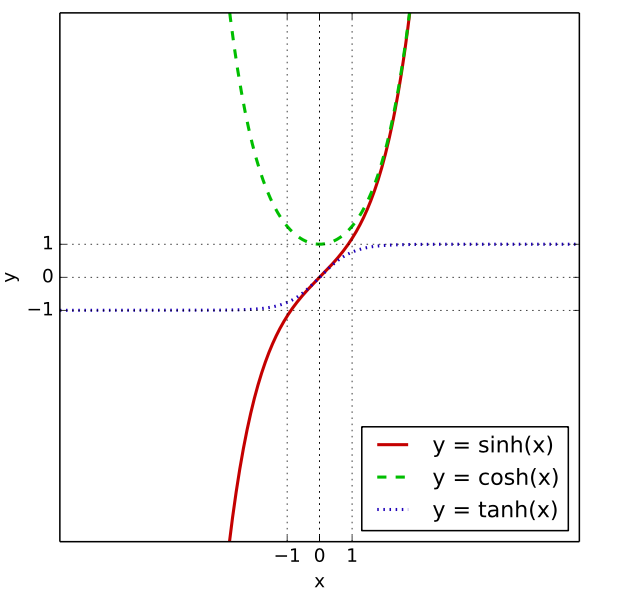
\includegraphics [scale=0.35] {sinhcosh.png} \end{center}
Notice that $\cosh$ is never zero, while only $\sinh 0 = 0$.

So if we look again at 
\[ \sin z = \sin x \cosh y + i \cos x \sinh y \]
and ask, where is this function equal to zero?  

Both parts must vanish.  Since $\cosh$ is never zero, $\sin x$ must be zero.  This happens for $x = 2k \pi$.  

The cosine of this $x$ is equal to $1$, that means $\sinh y$ must be $0$ which only happens for $y = 0$.

So the zeroes of the complex sine function are at $z = 2k \pi + 0i$.

Alternatively, go back to the original definition:
\[ \sin z = \frac{1}{2i} (e^{iz} - e^{-iz}) \]
which vanishes only for 
\[ e^{iz} = e^{-iz} = \frac{1}{e^{iz}} \]
\[ e^{2iz} = \ [ \ e^{iz} \ ]^2 \ = 1 \]
\[ e^{iz} = \pm 1 \]
\[ e^{i(x + iy)} = \pm 1 \]
\[ e^{-y}e^{ix} = \pm 1 \]
\[ e^{-y} (\cos x + i \sin x) = \pm 1 \]
The imaginary part must be zero, so $x = 2k \pi$.  The other part must be equal to $\pm 1$, so $y = 0$ and $\cos 2k \pi = 1$, which works.

For the cosine
\[ \cos z = \frac{1}{2i} (e^{iz} + e^{-iz}) \]
This is equal to zero when
\[ e^{iz} = - e^{-iz} = -\frac{1}{e^{iz}} \]
\[ e^{2iz} = -1 \]
\[ e^{i(x + iy)} = \pm i \]
\[ e^{-y} (\cos x + i \sin x) = \pm i \]
In this case we need $\cos x = 0$ and then $y=0$ and $\sin x = 1$ will work.  $x = (2k + 1)\pi / 2$.

Recall that
\[ \cos z = \cos x \cosh y - i \sin x \sinh y \]
Since $\cosh$ is never zero, $\cos x$ must be zero.  Then either $\sin x = 0$ or $\sinh y = 0$.  Only the latter works for the non-imaginary part, so we have that $y = 0$.

\subsection*{analyticity}
We proved before that the complex exponential is analytic.  There is a theorem that says that if we add two analytic functions together, the result is also analytic.  Hence, the trigonometric functions are analytic.

But, just to check this result, let's write them out in terms of $u$ and $v$ and see whether the partial derivatives follow the CRE conditions:

\[ \sin z = \sin x \cosh y + i \cos x \sinh y \]
Taking the derivatives:
\[ u(x,y) =  \sin x \cosh y \]
\[ u_x = \cos x \cosh y \]
\[ u_y = \sin x \sinh y \]
and
\[ v(x,y) = \cos x \sinh y \]
\[ v_x = - \sin x \sinh y \]
\[ v_y = \cos x \cosh y \]
So we see that
\[ u_x = v_y \]
\[ u_y = -v_x \]

The CRE are satisfied and therefore, the complex sine is analytic.

Similarly we have that 
\[ \cos z = \cos (x + iy) \]
\[ = \cos x \cos iy - \sin x \sin iy \]
\[ = \cos x \cosh y - i \sin x \sinh y \]
So
\[ u(x,y) =  \cos x \cosh y \]
\[ u_x = - \sin x \cosh y \]
\[ u_y = \cos x \sinh y \]
and
\[ v(x,y) = -\sin x \sinh y \]
\[ v_x = -\cos x \sinh y \]
\[ v_y = -\sin x \cosh y \]
So we see that
\[ u_x = v_y \]
\[ u_y = v_x \]
Thus the complex cosine is also analytic.

We can also prove that:

\[ \sin^2 z + \cos^2 z = 1 \]
The easy way is
\[ \cos^2 z + \sin^2 z = \ [ \frac{e^{iz} + e^{-iz}}{2} \ ]^2 +  [ \frac{e^{iz} - e^{-iz}}{2i} \ ]^2 \ ] \]
\[= \frac{e^{2iz} + 2 + e^{-2iz} - e^{2iz} + 2 - e^{-2iz} }{4} \]
\[ = 1 \]

\section{CRE}
The function
\[ f(x,y) = \frac{x^2}{x^2 + y^2} \]
has some problems:  first, it is not defined at the origin $(0,0)$ but also, as we approach the origin along the $x$-axis and the $y$-axis we get different limiting values, namely
\[ f(x,0) = \frac{x^2}{x^2} = 1 \]
\[ f(0,y) = \frac{0}{y^2} = 0 \]

Rewriting it in polar coordinates ($x = r \cos \theta, r^2 = x^2 + y^2$):
\[ f(r,\theta) = \frac{r^2 \cos^2 \theta}{r^2} = \cos^2 \theta \]

Shankar says:  the function $f$ is generally a function of \emph{two} complex variables, $z$ and its complex conjugate:
\[ z = x + iy \]
\[ z* = x - iy \]
which can be written in terms of $x$ and $y$ as
\[ x = \frac{z + z*}{2} \]
\[ y = \frac{z - z*}{2i} \]
Generally, the value of $f$ depends on both $z$ and $z*$, but we will be very interested in functions which depend only on $z$ and not $z*$.  The reason for this is that only such functions have the property that the derivative at a point does not depend on the direction from which we approach that point.

Consider the function:
\[ f(x,y) = x^2 - y^2 \]
\[ = \frac{(z+z*)^2}{4} + \frac{(z-z*)^2}{4} \]
\[ = \frac{1}{4} \ [ \ z^2 + 2zz* + z*^2 + z^2 - 2zz* + z*^2 \ ] \]
\[ = \frac{z^2 + z*^2}{2} \]
This function is not a function only of $z$ but of both $z$ and $z*$.

We say that $f$ is an \emph{analytic} function of $z$ if it does not depend on $z*$.  Shankar says this means that "$x$ and $y$ enter $f$ \emph{only} in the combination $x + iy$".

The famous Cauchy-Riemann Equations (CRE) are true for $f \iff f$ is an analytic function of $z$.  

For:
\[ f(x,y) = u(x,y) + iv(x,y) \]
The CRE conditions are:
\[ u_x = v_y \]
\[ u_y = -v_x \]

Consider:
\[ f(x,y) = x^2 - y^2 + i2xy \]
CRE requires
\[ u_x = 2x \stackrel{?}{=}  v_y = 2x \]
\[ v_x = 2y \stackrel{?}{=} - u_y = 2y \]
The function is analytic.  As Shankar says, this is expected because:
\[ x^2 - y^2 + 2ixy = (x + iy)(x + iy) = z^2 \]

Consider:
\[ f(x,y) = \cos y - i \sin y \]
CRE requires:
\[ u_x = 0 \stackrel{?}{=} v_y = - \cos y \]
\[ v_x = 0 \stackrel{?}{=}  -u_y = - \sin y \]
This is "impossible" since there is no $y$ that satisfies both of the conditions.  And it's not surprising since
\[ y = \frac{z - z*}{2i} \]

Consider:
\[ f(x,y) = x^2 + y^2 \]
CRE requires:
\[ u_x = 2x \stackrel{?}{=}  v_y = 2y \]
\[ u_y = 0 \stackrel{?}{=}  -v_x \]
CRE are only satisfied if $x=y$.  Also not surprising since
\[ x^2 + y^2 = zz* \]

Consider:
\[ f(x,y) = x^2 - y^2 \]
CRE requires:
\[ u_x = 2x \stackrel{?}{=} v_y = -2y \]
which is true if $x = y$.
\[ u_y = 0 \stackrel{?}{=} -v_x = 0 \]
But "no importance is given to functions which obey the CRE only at isolated points or on lines."

Consider:
\[ f(x,y) = e^x \cos y + i e^x \sin y \]
CRE requires:
\[ u_x = e^x \cos y \stackrel{?}{=} v_y = e^x \cos y \]
\[ u_y = -e^x \sin y \stackrel{?}{=} -v_x = - \sin y e^x \]
Both are true, so this one does satisfy CRE.

Shankar doesn't mention it here but the last function is special, it is $f(z) = e^z$:
\[ e^x \cos y + i e^x \sin y \]
\[ = e^x (\cos y + i \sin y) \]
\[ = e^x e^{iy} \]
\[ = e^{x + iy} \]
\[ = e^z \]
and we did this one in the previous section.

For functions of interest, it may often be true that CRE fails at particular points called \emph{singularities}.

Consider:
\[ f(x,y) = \frac{1}{z} = \frac{z*}{zz*} = \frac{x-iy}{x^2 + y^2} \]
We need:
\[ u_x = \frac{d}{dx} \ \frac{x}{x^2 + y^2} = \frac{x^2 + y^2 - 2x^2}{(x^2 + y^2)^2}  = \frac{y^2 - x^2}{(x^2 + y^2)^2} \]
\[ v_y = \frac{d}{dy} \ (-\frac{y}{x^2 + y^2} ) = - \frac{x^2 - y^2}{(x^2 + y^2)^2} = u_x \]
\[ u_y =  0 = v_x \]
But the function blows up at the origin.  This described by saying it has a pole at the origin.
The function
\[ f(z) = \frac{c}{z} \]
where $c$ is a constant, also blows up at the origin.  We say that the \emph{residue} of the pole at the origin is $c$.

\section{Integrate}
Complex functions are differentiated and integrated in a way that is similar to real functions, with these differences:  normally, we restrict our attention to functions that are analytic, and we pay attention to points in the complex plane where they have poles (or singularities).  

Also, the integrals that we compute are line integrals.  Let's do one.

\subsection*{example}

In general terms, if we have
\[ z = x + i y \]
\[ dz = dx + i dy \]
and the function
\[ w = f(z) \]
\[ = u(x,y) + iv(x,y) \]
we can write either
\[ \int f(z) \ dz = \int (x + i y) (dx + i dy) \]
or what may be less confusing:
 \[ \int f(z) \ dz = \int (u + i v) (dx + i dy) \]
\[ = \int (u + iv) \ dx + (- v + i u) \ dy \]
\[ = \int u \ dx - v \ dy + iv \ dx + iu \ dy \]

The integral of a complex function is defined as a sum of integrals of two real variables.  Just as with line integrals for real functions of $x$ and $y$, the variables are related by the curve over which we will integrate.

Recall that for the work integral
\[ \int_C \mathbf{F} \cdot d \mathbf{r} = \int_C M \ dx + N \ dy \]
we parametrize the curve to get the integral over a single variable.

We can view $y$ as a function of $x$ or perhaps, we can parametrize both $x$ and $y$ as functions of $t$.

Suppose our function is simply $z = x + iy$.  The integral is 
\[ \int z \ dz = \int (x + iy) (dx + i dy) \]
\[ = \int x \ dx - y \ dy + i x \ dy + i y \ dx \]

Now we must get $y$ in terms of $x$ from the curve.  Suppose the curve goes from $(1,i)$ to $(3,i)$, then to $(3,3i)$ and finally back to where we started.  

We have three segments.  Along the first part, we are moving in the positive $x$ direction, with no change in $y$, so $dy=0$ and $y = 1$, a constant, and the integral is
\[ \int x \ dx - y \ dy + i x \ dy + i y \ dx \]
\[ = \int x \ dx + i y \ dx \]
\[ = \int_{x=1}^{x=3} \ x + i  \ dx \]
\[ = \frac{x^2}{2} + ix \ \bigg |_1^3 \]
\[ = 4 + 2i \]

Along the second part, we are moving in the positive $y$ direction with $dx = 0$ and $x = 3$ so
\[ \int x \ dx - y \ dy + i x \ dy + i y \ dx \]
\[ = \int_{y=1}^{y=3} - y \ dy + 3 i \ dy \]
\[ = -\frac{y^2}{2} + 3iy \ \bigg |_1^3 \]
\[ = -4 + 6i \]

And for the third, both $dx$ and $dy$ are non-zero, so we must actually do the parametrization.  The curve is $y=x$.  Hence $dy = dx$.
\[ \int x \ dx - y \ dy + i x \ dy + i y \ dx \]
\[ = \int x \ dx - x \ dx + i x \ dx + i x \ dx \]
\[ = 2i \int x \ dx \]
Consider first the direction of the path as going from $(1,1)$ to $(3,3)$.
\[ = 2i \int_{x=1}^{x=3} x \ dx \]
\[ = 2i \ \frac{x^2}{2} \ \bigg |_1^3 \]
\[ = 2i \ \frac{8}{2} = 8i \]
However, for the closed path, where we end up back at the starting point, $C3$ should be moving from $(3,3)$ to $(1,1)$ so we have 
\[ 2i \ \frac{x^2}{2} \ \bigg |_3^1 = 2i \ - \frac{8}{2} = -8i \]
Notice that 
\[ \int_{C1} + \int_{C2} = 8i  = - \int_{C3}\]
If we follow the curve $C3$ from $(3,3)$ to $(1,1)$, the whole thing is just zero.  Later we'll see that this is not a coincidence.

\subsection*{example}
Suppose the function is
\[ f(z) = y - x - i3x^2 \]
and we proceed from the origin to the point $z = 1 + i$ either directly ($C_2$) or by first going up vertically and then across ($C_1$).

For the vertical part of $C_1$ we have that $x = 0$ and $dx = 0$.
\[ I = \int ( y - x - i3x^2 )\ (dx + idy) \]
\[ = \int y i \ dy \]
It's important to recognize that although we are proceeding from the point $z=0$ to the point $z = i$, the upper bound on this integral is not $i$ but $y = 1$!  Hence
\[ I = i\frac{y^2}{2} \ \bigg |_0^1 = \frac{i}{2} \]
For the horizontal part of $C_1$ we have that $y=1$ and $dy = 0$ so
\[ I = \int ( y - x - i3x^2 )\ (dx + idy) \]
\[ = \int (1 - x - i3x^2) \ dx \]
\[ = x - \frac{x^2}{2} - ix^3 \ \bigg |_0^1 = \frac{1}{2} - i \]
Therefore the total
\[ I = \frac{i}{2} + \frac{1}{2} - i = \frac{1}{2} \ (1 - i) \]
When going directly from the origin to $1 + i$ we relate $x$ to $y$ by the equation of the line $y=x$ so $dy = dx$ and
\[ I = \int ( y - x - i3x^2 )\ (dx + idy) \]
\[ = \int - i3x^2 \ (dx + i dx) \]
\[ = -i  \ x^3 \ \bigg |_0^1 + x^3 \ \bigg |_0^1 = -i \cdot 1 + 1 = 1  - i \]
And around the closed curve going backward along $C_2$:
\[ \oint f(z) \ dz =  \frac{1}{2} \ (1 - i) - (1  - i ) = -\frac{1}{2} (1 + i) \]

\section{Integrate}
If the contour (curve) of integration $C$ is parametrized in terms of $t$, then
\[ \int_C f(z) \ dz = \int_a^b f[z(t)] \ z'(t) \ dt \]

A particularly important parametrization is for circular paths.  On such a path, $z$ takes on values with constant $r$ and the only change is in $\theta$.  So we have
\[ z = re^{i \theta} \]
\[ z'(\theta) = i z \]
\[ dz = i z \ d \theta \]

As an example, consider $f(z) = z*$.

Note that this function is \emph{not} analytic, because it involves $z*$ rather than $z$, and secondly because
\[ z* = x - iy \]
so
\[ u_x = 1\ , \ \ \  v_y = - 1 \]
\[ u_x \ne v_y \]
The CRE do not hold.

Suppose our curve is the circle of radius $r$ centered at the origin, and we proceed between the endpoints $z = -ri \rightarrow ri$.  On this half-circle 
\[ z = re^{i \theta} \]
we have then
\[ dz = i \ re^{i \theta} \ d \theta \]
In radial coordinates
\[ z* = re^{-i\theta} \]
so we have
\[ \int {z*} \ dz = \int r e^{-i\theta} r i e^{i \theta} \ d \theta \]
\[ = r^2 i \int_{-\pi/2}^{\pi/2} d \theta = r^2 \pi i \]
Alternatively,
\[ zz* = |z|^2 = r^2  \]
\[ z* = \frac{r^2}{z} \]
\[ \int {z*} \ dz = r^2 \int \frac{1}{z} \ dz \]
Again
\[ z = re^{i \theta} \]
\[ dz = iz \ d \theta \]
So the integral is just
\[ = r^2 \int \frac{1}{z} \ iz \ d \theta   \]
\[ = r^2 i \int d \theta = r^2 \pi i \]

\subsection*{example}
Consider $f(z) = z^2$.  For the path, take the unit circle over the first quadrant from $(1,0)$ to $(0,1)$.  There is an easy way to do this, and a hard way.  Let's start by checking that this function is analytic, and then doing the hard way first.

Write $z$ in terms of $x$ and $y$:
\[ z = x + iy \]
\[ z^2 = (x + iy)^2 = x^2 - y^2 + i2xy \]
\[ u_x = 2x = v_y \]
\[ u_y = -2y = -v_x \]
The CRE hold.

Also
\[ dz = dx + i \ dy \]
So
\[ \int z^2 \ dz = \int (x^2 - y^2 + 2ixy) ( dx + i \ dy) \]
\[ = \int (x^2 - y^2) \ dx - \int 2 xy \ dy + i \int 2xy \ dx + i \int (x^2-y^2) \ dy \]
As before, we must parametrize this using the relationship between $x$ and $y$ along the curve.
\[ x = \cos t \]
\[ y = \sin t \]
\[ dx = - \sin t \ dt \]
\[ dy = \cos t \ dt \]
and then
\[ x^2 - y^2 = \cos^2 t - \sin^2 t = \cos 2t \]
\[ 2xy = 2 \cos t \sin t = \sin 2t \]
so the integral is
\[ = \int -\cos 2t \  \sin t \ dt - \int \sin 2t \ \cos t \ dt + \dots \]
\[ + \ i \ [ \ \int - \sin 2t \ \sin t \ dt + \int \cos 2t \ \cos t \ dt \]

Looks pretty wild!  In the book they use some trig identities I hadn't seen before, namely starting with the standard
\[ \sin s + t = \sin s \cos t + \sin t \cos s  \]
\[ \cos s + t = \cos s \cos t - \sin s \sin t \]
then, if $s = 2t$ then
\[ \sin 3t = \sin 2t \cos t + \sin t \cos 2t \]
\[ \cos 3t = \cos 2t \cos t - \sin 2t \sin t \]
Looking at the real part of the integral we had (combining terms)
\[ \int -\cos 2t \  \sin t - \sin 2t \ \cos t \ dt = \int - \sin 3t \ dt = \frac{\cos 3t}{3} \]
and for the imaginary part of the integral
\[ i \ [ \ \int - \sin 2t \ \sin t + \cos 2t \ \cos t \ dt = i \int \cos 3t \ dt = i \ \frac{\sin 3t}{3} \]
That looks a lot better.
\[ \frac{\cos 3t}{3} + i \ \frac{\sin 3t}{3} \ \bigg |_0^{\pi/2} = - \frac{1}{3} - i \ \frac{1}{3} = - \frac{1}{3} (1 + i) \]

For the easy way, just treat $z$ as if it were a real variable
\[ \int z^2 \ dz = \frac{z^3}{3} \ \bigg |_1^i = - \frac{1}{3} i - \frac{1}{3} \]
Note that if we go all the way around the unit circle the integral is just zero.

Going back to the first example we had
\[ \int z \ dz = \frac{z^2}{2} \ \bigg |_{1 + i}^{3 + 3i} \]
\[ = \frac{9 - 9 + 18i - \ [ \ 1 - 1 + 2i \ ] }{2} \]
\[ = 8i \]

\subsection*{example}
\[ \int_0^{2\pi} \frac{1}{z} \ dz \]

Examining the inverse function, let's first confirm that it is analytic by calculating the partial derivatives.  We have
\[ \frac{1}{z} = \frac{1}{x + iy} \]
Simplify by multiplying on top and bottom by $z*$:
\[ = \frac{1}{x + iy} \ \frac{x-iy}{x- iy} \]
\[ = \frac{x - iy}{x^2 + y^2} \]
Thus
\[ u = \frac{x}{x^2 + y^2} \]
\[ u_x = \frac{(x^2 + y^2) - 2x^2}{(x^2 + y^2)^2} = \frac{y^2 - x^2}{(x^2 + y^2)^2} \]
\[ u_y = \frac{-2xy}{(x^2 + y^2)^2} \]
And
\[ v =  \frac{-y}{x^2 + y^2} \]
\[ v_y = - \frac{(x^2 + y^2) - 2y^2}{(x^2 + y^2)^2} = \frac{y^2 - x^2}{(x^2 + y^2)^2} \]
\[ v_x = \frac{2xy}{(x^2 + y^2)^2} \]
CRE are satisfied and the inverse of $z$ is indeed analytic.

If we are on the unit circle, then 
\[ z = e^{i\theta} \]
\[ dz = ie^{i\theta} d \theta = iz\ d \theta \]
\[ \int \frac{dz}{z} = \int \frac{iz}{z} \ d \theta = 2 \pi i \]

If we're centered on the origin but we don't have a unit circle, there will be an $R$ in both the numerator and the denominator, which cancel.

The result is thus independent of the radius of the circle.

In general
\[ \oint_C \frac{dz}{(z - z_0)^n} = 
\begin{cases}
0, & n \ne 1 \\
2 \pi i, & n = 1 
\end {cases}
\]
(We will see examples for $n \ne 1$ below).

We can also integrate the inverse function in terms of $x$ and $y$:
\[ \oint \frac{1}{z} \ dz = \oint \frac{dx + i dy}{x + iy} \]
\[ = \oint \frac{1}{x^2+y^2} \ [ \  x \ dx - y \ dy + i x \ dy + i y \ dx \ ] \]
Suppose we go on a circle of radius $R$ centered on the origin and parametrize in terms of $\theta$.  We obtain:
\[ x = R \cos \theta \]
\[ y = R \sin \theta \]
\[ x^2 + y^2 = R^2 \]
\[ dx = - R \sin \theta \ d \theta \]
\[ dy = R \cos \theta \ d \theta \]
We have for the integral
\[ \oint \frac{1}{x^2+y^2} \ [ \  x \ dx - y \ dy + i x \ dy + i y \ dx \ ] \]
\[ = \int \frac{1}{R^2} \ [ \ -R^2 \cos \theta \sin \theta \ d \theta + R^2 \sin \theta \cos \theta \ d \theta + i R^2 \cos^2 \theta \ d \theta + i R^2 \sin^2 \theta \ d \theta \ ] \]
\[ = \int \frac{1}{R^2} \ [ \ i R^2 \cos^2 \theta \ d \theta + i R^2 \sin^2 \theta \ d \theta \ ] \]
\[ = \int \frac{1}{R^2} \ [ \ i R^2 \ d \theta \ ] \]
\[ = \int i \ d \theta = 2 \pi i \]

Note that if we integrate the same function around a unit square, we run into problems.  First let's  do $[0,0 \times 1,1]$.  We have
\[ \int u \ dx - \int v \ dy + i \ [ \ \int v \ dx + \int u \ dy \ ]  \]
Along $C1$, $y = 0$ and $dy = 0$ so:
\[ \int \frac{x}{x^2 + y^2} \ dx + i \ [ \ \int \frac{-y}{x^2 + y^2} \ dx \]
\[ = \int_0^1 \frac{1}{x} \ dx = \ln x \ \bigg |_0^1 \]
Since $\ln 0$ is not defined, we can't do this.

Logarithms are tricky, no doubt.  If the complex logarithm $Log z$ is defined and differentiable along the curve (say the semicircle from $-i$ to $i$), we can do this:
\[ I = \int_{-i}^i \frac{1}{z} \ dz = \text{ Log } z \ \bigg |_{-i}^i  \]
Recall that $z = re^{i\theta}$ with $r=1$ so this is
\[ = (\ln 1 + i \ \frac{\pi}{2} ) - (\ln 1 + i \frac{-\pi}{2} ) = 2i \ \frac{\pi}{2} = \pi i \]
For any value of $r$ (except $r=0$), we get the same answer, since $\ln r - \ln r = 0$.

\subsection*{example}
We can extend this to 
\[ \oint \frac{1}{z^2} \ dz \]
As before, on the unit circle
\[ z = e^{i\theta} \]
\[ dz = i z \ d \theta \]
so the integral is
\[ \int_0^{2 \pi} \ \frac{i}{z} \ d \theta =  \int_0^{2 \pi} i e^{-i\theta} \ d \theta \]
Now
\[ \int e^{-i\theta} \ d \theta = -i e^{-i\theta} \]
so cancel $i \cdot -i$ and we have just
\[ = e^{-i\theta} \ \bigg |_0^{2 \pi}  \]
Evaluate the first term using Euler's formula:
\[ e^{-2\pi i} = \cos -2 \pi + i \sin -2 \pi \]
\[ = \cos 2 \pi - i \sin 2 \pi = 1 \]
So the whole thing is zero.

In fact, for any negative integer power of $z$
\[ \int z^{-n} \ dz \]
around the unit circle $z=e^{i\theta}$ we have
\[ i \int e^{-i(n-1)\theta} \ d \theta \]
\[ = \frac{1}{n-1} \ e^{-i(n-1)\theta} \ \bigg |_0^{2 \pi}  \]
\[ = \frac{1}{n-1} \ [ \ (\cos 2 (n-1) \pi - i \sin 2 (n-1) \pi ) \ - 1 ]   \]
\[ = \frac{1}{n-1} \ [ \ 1  - 1 ] \ = 0  \]

\subsection*{example}
Consider
\[ \int \sqrt{z} \ dz \]
along the half-circle of radius $3$ starting from the point $z = R$ on the $x$-axis and proceeding counter-clockwise.
We can do this integral even if the "branch" of the square root function that we're using is only defined for $\theta > 0$.  We have that 
\[ z = Re^{i\theta}, \ \ \ \theta = 0 \rightarrow \pi \]
\[ dz = iz = iRe^{i\theta} \ d \theta \]
\[ \sqrt{z} = \sqrt{R} e^{i\theta/2} \]
so
\[ I = \int_0^{\pi} iR \sqrt{R} e^{i3\theta/2} \ d \theta \]
We need
\[ \int e^{i3\theta/2} \ d \theta = \frac{2}{3i} e^{i3\theta/2} \ \bigg |_0^{\pi} \]
easiest to write it out as
\[ e^{i3\theta/2} \ \bigg |_0^{\pi} = \cos \frac{3\pi}{2} + i \sin  \frac{3\pi}{2} - \cos 0 - i \sin 0 \]
\[ = 0 + i(-1) - 1 - 0 = -(1+i) \]
Going back to pick up all the factors we left behind:
\[ I = -iR \sqrt{R} \ \frac{2}{3i} \ (1+i) = -R \sqrt{R} \ \frac{2}{3} \ (1+i) \]
In the problem, $R$ was actually specified as $3$, leading to the cancellation:
\[ I = - 2 \sqrt{3} \ (1+i) \]

We can also do this problem by antiderivatives:
\[ \int_R^{-R} \sqrt{z} \ dz = \frac{2}{3} \ z^{3/2} \ \bigg |_R^{-R}  \]
\[ = \frac{2}{3} ( R^{3/2} e^{i3\pi/2} - R^{3/2} e^0) \]
\[ = \frac{2}{3} R^{3/2} ( e^{i3\pi/2} - 1) \]
and, as we showed above:
\[ e^{i3\pi/2} = -i \]
If $R=3$ we get the same answer as before.

\section{Cauchy}
Cauchy's first theorem says that the integral of an analytic function over a closed path is equal to zero, when the enclosed region does not contain a singularity.
\[ \oint_C f(z) \ dz = 0 \]
This will turn out to be a consequence of Green's Theorem, which you should remember from multivariable calculus.  Let
\[ z = x + i y \]
\[ dz = dx + i dy \]
\[ z = f(x,y) = u(x,y) + iv(x,y) \]
Our integral is
\[ \oint z \ dz = \oint (u(x,y) + iv(x,y)) \ (dx + i dy) \]
\[ =  \oint u(x,y) \ dx - \oint v(x,y) \ dy + i \oint v(x,y) \ dx + i \oint u(x,y) \ dy \]
As before, because we are moving along a curve there is a relationship between $x$ and $y$, so we can either express that relationship (for say, $y$ in terms of $x$), or parametrize the curve in terms of $t$ or $\theta$.  In either case, these become integrals in a single variable.  We suppress the $(x,y)$ notation and the extra integral signs:
\[ =  \oint u \ dx - v \ dy + i v \ dx + i u \ dy \]

\subsection*{proof of Cauchy 1}
Back in vector calculus we proved Green's theorem, which says that for two real functions of $x$ and $y$:  $M(x,y)$ and $N(x,y)$:
\[ \oint_C M dx + N dy = \iint_R (\frac{\partial N}{\partial x} - \frac{\partial M}{\partial y}) \ dx \ dy \]
Back then, $M$ and $N$ were components of a vector field $\mathbf{F}$ and we wrote the shorthand for curl:
\[ = \iint_R \nabla \times \mathbf{F} \ dA\]
but the important thing is that they are real-valued functions of two real variables $f: \mathbb{R}^2 \rightarrow \mathbb{R}^1$.

In terms of $u$ and $v$ we have for the real part of Cauchy's Theorem that $M=u$ and $N = -v$ (notice the minus sign!).  

So:
\[ \oint u \ dx - v \ dy = \iint_R (-\frac{\partial v}{\partial x} -  \frac{\partial u}{\partial y}) \ dx \ dy \]
\[ = - \iint_R (v_x + u_y) \ dx \ dy \]
But, according to the CRE
\[ u_y = -v_x \]
Hence, this integral is zero.

For the imaginary part we use Green's Theorem again with $N=u$ and $M = v$ (no minus sign here):
\[ \oint v \ dx + u \ dy =  \iint_R (\frac{\partial u}{\partial x} - \frac{\partial v}{\partial y}) \ dx \ dy \]
\[ =  \iint_R (u_x - v_y) \ dx \ dy \]
But, again, according to the CRE
\[ u_x = v_y \]
So the integral for the imaginary part is also zero, and thus the whole thing is zero as well:
\[ \oint u \ dx - \oint v \ dy + i \oint v \ dx + i \oint u \ dy = 0 \]

Remember how important it was (for Green's theorem) that the function being integrated be defined everywhere in the region.  Well, it's true here as well.

\[ \oint_C \frac{1}{z} \ dz \stackrel{?}{=} 0 \]

We've already seen by direct calculation that this integral is \emph{not} zero when the curve $C$ includes the origin, but it \emph{is} zero otherwise.

To repeat the demonstration for the former case we use the unit circle centered at the origin.  Write
\[ z = r e^{i\theta} \]
\[  \frac{dz}{d\theta} = r i e^{i\theta} = iz \]
Hence
\[ \oint_C \frac{1}{z} \ dz = \oint_C \frac{1}{z} \ iz \ d \theta \]
\[ = i   \oint_C  d \theta = 2 \pi i \]

\subsection*{Path independence}
The theorem that says the integral of an analytic function over a closed path (over a region without a singularity), is equal to zero.
\[ \oint_C f(z) \ dz = 0 \]

This result means, in turn, that the integral of an analytic function between two points $z_1$ and $z_2$ is independent of the path taken.  Call the two paths $C1$ and $C2$.  

Form the closed path by going from $z_1$ to $z_2$ over $C1$ and then return to $z_1$ by going backward over $C2$.  The total integral is equal to zero by Cauchy's Theorem.
\[ \int_{C1} f(z) \ dz + \int_{-C2} f(z) \ dz = 0 \]
But the integral over the path $C_2$ in the forward direction is just minus the integral over the reverse path $-C2$.
\[ \int_{-C2} f(z) \ dz = - \int_{C2} f(z) \ dz \]
Thus
\[ \int_{C1} f(z) \ dz - \int_{C2} f(z) \ dz = 0 \]
and
\[ \int_{C1} f(z) \ dz = \int_{C2} f(z) \ dz \]

\subsection*{example}

We will integrate the function $f(z) = z$ over a rectangle ($R = [0,a] \times [b,0]$.  Write
\[ z = x + i y \]
\[ dz = dx + i dy \]
\[ f(x,y) = u(x,y) + iv(x,y) \]
Our integral is
\[ \int z \ dz = \int (u + iv) \ (dx + i dy) \]
\[ = \int u \ dx - \int v \ dy + i \int v \ dx + i \int u \ dy \]
Since the whole thing is equal to zero over our closed path, both parts are equal to zero:
\[ \int u \ dx - \int v \ dy = 0 \]
\[ \int v \ dx + \int u \ dy = 0 \]
Does this look familiar?

\subsection*{application of Cauchy 1}

The function we'll be working with is one we introduced before:
\[ u(x,y) =  e^{-x^2} e^{y^2} \cos 2xy \]
\[ v(x,y) = e^{-x^2} e^{y^2} (- \sin 2xy) \]
Everything will simplify pretty quickly.  Divide the path into its four parts and compute each separately:
Over $C1$, $y=0$ and $dy = 0$ so we have:
\[ \int_{C1} = \int u \ dx = \int_0^a e^{-x^2} e^{0} \cos 0 \ dx = \int_0^a e^{-x^2} \ dx \]
C2 ($x = a$, $dx = 0)$:
\[ \int_{C2} = - \int_0^b e^{-a^2} e^{y^2} (- \sin 2ay) \ dy  \]
C3 ($y = a$, $dy = 0)$:
\[ \int_{C3} = \int_a^0 e^{-x^2} e^{b^2} (\cos 2bx) \ dx  \]
C4 ($x = 0$, $dx = 0$):
\[ \int_{C4} = \int_b^0 e^{y^2} (-\sin 0) \ dy = 0 \]
So all together:
\[ \int_0^a e^{-x^2} \ dx - \int_0^b e^{-a^2} e^{y^2} (- \sin 2ay) \ dy + \int_a^0 e^{-x^2} e^{b^2} \cos 2bx \ dx = 0 \]
\[ \int_0^a e^{-x^2} \ dx = e^{-a^2} \int_0^b e^{y^2} (- \sin 2ay) \ dy + e^{b^2} \int_0^a e^{-x^2} \cos 2bx \ dx  \]
Let $a \rightarrow \infty$.  Then
\[ e^{-a^2} \rightarrow 0 \]
so the first term on the right side goes to zero and we have:
\[ \int_0^{\infty} e^{-x^2} \ dx = e^{b^2} \int_0^{\infty} e^{-x^2} \cos 2bx \ dx  \]
But we know the value of the left-hand side, it is 
\[ \int_0^{\infty} e^{-x^2} \ dx = \frac{\sqrt{\pi}}{2} \]
so
\[  \int_0^{\infty} e^{-x^2} \cos 2bx \ dx = \frac{\sqrt{\pi}}{2} \ e^{-b^2} \]
The Gaussian that we know, is a special case of this general form.

\section{Cauchy}
If we can write an integral as
\[ \oint_{C} \frac{f(z)}{z-z_0} \ dz \]
where $f(z)$ is analytic and defined everywhere in the domain we care about, then we will show that the value of this integral is 
\[ \oint_C \frac{f(z)}{z-z_0} \ dz = 2 \pi i f(z_0) \]

\subsection*{derivation of Cauchy 2}
Suppose $f(z)$ is analytic and defined everywhere within some region \emph{except} at a singularity, $z_0$.  For example, suppose we have
\[ \frac{f(z)}{z-z_0} \]
We integrate this function around a special closed path in the region of analyticity:
\[ \oint \frac{f(z)}{z-z_0} \ dz \]
\begin{center} 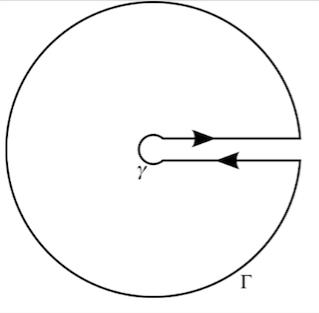
\includegraphics [scale=0.5] {keyhole.png} \end{center}
It's not labeled but the singularity $z_0$ is at the center of the two concentric circles.  The "keyhole" excludes $z_0$ so $f$ is analytic everywhere in the region enclosed by the path.

Cauchy's first theorem tells us that the total integral is zero.

The straight line segments are so close to each other as to be equal, but traversed in opposite directions, so the net contribution from them is zero.

Therefore by Cauchy 1 we have that the integral around the outer ring counter-clockwise + the integral around the inner ring clockwise add up to zero.

But reversing the direction of integration on the inner ring (so both paths go in the counter-clockwise direction) changes the sign of the value, hence we have that
\[ \oint_{C \ \text{outer}} \frac{f(z)}{z-z_0} \ dz - \oint_{C \ \text{inner}} \frac{f(z)}{z-z_0} \ dz = 0 \]
and
\[ \oint_{C \ \text{outer}} \frac{f(z)}{z-z_0} \ dz = \oint_{C \ \text{inner}} \frac{f(z)}{z-z_0} \ dz \]

Notice that we haven't said anything about the radius of these rings.  

What this means is that the value of the integral around a ring enclosing a singularity is not zero, but is independent of the radius.

We can parametrize this path by realizing that each point on one of these curves is given by
\[ z = z_0 + \rho e^{i\theta}, \ \ \ 0 \le \theta \le 2 \pi \]

Since $z_0$ is a constant
\[ dz = i \rho e^{i \theta} d \theta \]
But
\[ z - z_0 = \rho e^{i\theta} \]
so, substituting for $\rho e^{i\theta}$ above we obtain
\[ dz = i(z - z_0) \ d \theta \]
and
\[ \oint \frac{f(z)}{z - z_0} \ dz = \oint f(z) \ i \ d \theta \]
\[ = i \int_0^{2\pi}  f(z) \ d \theta \]

This holds for every circular path enclosing $z_0$.  We may choose $\rho$ as small as we like, and so we choose it very small ($\rho \rightarrow 0$) so
\[ f(z) \rightarrow f(z_0) = \text{constant} \]
and since it's constant we can bring it out from under the integral sign!
\[  \oint \frac{f(z)}{z - z_0} \ dz = i \int_0^{2\pi}  f(z) \ d \theta \] 
\[ = i f(z_0) \int_0^{2\pi} d \theta \]
\[ = 2 \pi i f(z_0) \]
What this means is that we can evaluate the integral in question by simply plugging in the value of the function at $z_0$ and multiplying that by $2 \pi i$.

\subsection*{examples}
Our formula is:
\[ \oint_{C} \frac{f(z)}{z-z_0} \ dz = 2 \pi i f(z_0) \]

A very simple example is:
\[ \oint_{C} \frac{1}{z} \ dz \]
Here $f(z) = 1$ and $z_0 = 0$ and the result should be
\[ I = 2 \pi i f(z_0) = 2 \pi i  \]
We computed this directly using the unit circle centered at $z = 0$.  We have that
\[ z = e^{i\theta} \]
\[ dz = i z \ d \theta \]
so
\[ \oint_{C} \frac{1}{z} \ dz = \int_0^{2 \pi}  \frac{1}{z} \ i z \ d \theta \]
\[ = \int_0^{2 \pi} i \ d \theta \]
\[ = 2 \pi i \]

\subsection*{translated from the origin}
Suppose we are interested in the value of the integral centered at a point $z_0 \ne 0$.  We consider those points $z$ in a circle constructed around $z_0$, that is
\[ z = z_0 + re^{it} \]
rearranging
\[ z - z_0 = re^{it} \]
We get the derivative of the polar form
\[ \frac{d}{dt} \ re^{it} = i re^{it}  \]
\[ = i(z-z_0) \]
Hence
\[ \int \frac{1}{(z-z_0)} \ dz  = \int \frac{1}{(z-z_0)} \ i(z - z_0) \ dt \]
\[ = 2 \pi i \]

However, we can also do this by Cauchy 2. The formula is
\[ \int \frac{f(z)}{z - z_0} \ dz = 2 \pi i \ f(z_0) \]
here the integrand is
\[ \frac{1}{(z-z_0)} \]
so $f(z)$ is just equal to $1$, and the answer is $2 \pi i$.

\section{P}
In a previous section, we showed that
\[ \oint_C \frac{f(z)}{z-z_0} \ dz = 2 \pi i f(z_0) \]
An example is
\[ \oint_C \frac{1}{z-z_0} \ dz = 2 \pi i \]

\subsection*{Residues}
By definition the residue at a simple pole $z_0$ is defined to be
\[ b_1 = \lim_{z \rightarrow z_0} (z-z_0) \ f(z)  \]
Just think of it as in the limit that $z \rightarrow z_0$, the denominator $z-z_0$ on the left of the first equation is a constant, so we can multiply both sides by $z - z_0$
\[  \oint \frac{f(z)}{z - z_0} \ dz = 2 \pi i f(z_0) \]
to obtain the result for the residue.
\[ \oint f(z) \ dz = 2 \pi i \ \lim_{z \rightarrow z_0} (z-z_0) \ f(z)  \]
using the definition
\[ b_1 = \lim_{z \rightarrow z_0} (z-z_0) \ f(z)  \]
we obtain
\[ \oint f(z) \ dz = 2 \pi i \ b_1  \]
If there is more than one such point
\[ \oint f(z) \ dz = 2 \pi i \ \sum \text{ Res } \]
The value of the integral is $2 \pi i$ times the sum of all the residues enclosed by the path.

\subsection*{Example 1}
This problem is Beck 4.26.  Consider 
\[ \oint f(z) \ dz = \oint \frac{1}{z^2 + 1} \ dz \]
We see that the denominator is zero when
\[ z^2 = -1 \]
\[ z = \pm \ i \]
Therefore we can factor the denominator as
\[ z^2 + 1 = (z + i) (z-i) \]

There are a couple of different ways to handle this.  One is to use partial fractions:
\[ \frac{1}{z^2 + 1} = \frac{1}{(z + i) (z-i)} \]
\[ = \frac{1}{2i} \ [ \ \frac{1}{z - i} - \frac{1}{z+i} \ ] \]
So the integral is a sum of two integrals:
\[ I = \frac{1}{2i} \ [ \oint \frac{1}{z - i}  \ dz -  \oint \frac{1}{z + i} \ dz \ ] \] 

Suppose the curve is the unit circle centered at $i$, designated as $C[i,1]$.  Obviously, this curve contains the singularity $z = i$.  The curve goes through the origin, so it does not extend as far as $z = -i$.

Therefore, the second integral is zero (no singularity) and the first is
\[ \frac{1}{2i} \ [ \ \oint \frac{1}{z - i}  \ dz \ ] \ = \frac{1}{2i} \ [ \  2 \pi i \ ] \]
by Cauchy 2.  Thus the value is just $I = \pi$

According to Beck, as an alternative, rewrite the function as
\[ \frac{1}{(z + i) (z-i)} = \frac{(1/z+i)}{z-i} \]
Thus
\[ \int \frac{1}{z^2 + 1} \ dz = \int \frac{(1/z+i)}{z-i} \ dz \]
We have essentially the same thing.

The function is
\[ \frac{1}{z+i} \]
and when evaluated at $i$, with result $1/2i$, we obtain
\[ \oint  \frac{f(z)}{z-z_0} \ dz = 2 \pi i \ f(z_0) \]
\[ = 2 \pi i \ \frac{1}{2i} = \pi \]

\subsection*{residues}
We do the same problem using residues.

We have
\[ b_1 = \lim_{z \rightarrow z_0} (z-z_0) \ f(z)  \]
and
\[ \oint f(z) \ dz = 2 \pi i \ b_1  \]
Evaluate the first equation:
\[ b_1 = \lim_{z \rightarrow z_0} (z-z_0) \ f(z)  \]
\[ = \lim_{z \rightarrow i} (z-i) \  \frac{1}{(z+i)(z-i)} \]
\[ = \frac{1}{2i} \]
And by the second equation:
\[ I = \pi \]
as before


If the unit circle had been centered at $-i$, rewrite the function as
\[ f(z) = \frac{1/z-i}{z+i} \]
The value of the function is
\[ \frac{1}{z-i}(-i) = -\frac{1}{2i} \]
and that integral is then $- \pi$.

A contour that includes both singularities integrates to zero.
\subsection*{partial fractions}
We can also do the curve containing both singularities by partial fractions.  Write
\[ \frac{1}{z^2 + 1} = \frac{1}{(z+i)(z-i)} \]
\[ = \frac{A}{z+i} + \frac{B}{z-i} \]
We need to determine $A$ and $B$.  When we multiply to put everything over the common denominator ($z^2 + 1)$ then for the numerators we will have:
\[ A(z-i) + B(z+i) = 1 \]
This gives
\[ Az + Bz = 0 \]
Hence $A = -B$.  And
\[ -Ai + Bi = 1 \]
\[ -Ai - Ai = -2Ai = 1 \]
\[ A = -\frac{1}{2i} \]
Hence the integrand is
\[ \frac{1}{z^2 + 1} = = \frac{A}{z+i} + \frac{B}{z-i} \]
\[ = -\frac{1}{2i(z+i)} + \frac{1}{2i(z-i)} \] 
For the curve including $z = i$ but not $z = -i$ we have that the left-hand integral is 0 by Cauchy's Theorem, and for the right hand side the function is
\[ f(z = z_0) = \frac{1}{2i} \]
So the value of the integral is
\[ 2 \pi i f(z_0) = 2 \pi i \ \frac{1}{2i} = \pi \]
as before.  The other pole we would have
\[ f(z = z_0) = -\frac{1}{2i} \]
and the result would be $- \pi$.  A curve enclosing both poles would have integral equal to zero.

\section{Residues}
Our formulas are:
\[ \oint_C \frac{f(z)}{z-z_0} \ dz = 2 \pi i f(z_0) \]
and
\[ b_1 = \lim_{z \rightarrow z_0} (z-z_0) \ f(z)  \]
\[ \oint f(z) \ dz = 2 \pi i \ b_1  \]
We worked one example using the method of residues in the previous section.  Here is where we get a lot more practice.



\subsection*{Examples}


\section{Series}
With this writeup, we'll start working through the last section of material on complex functions produced by the HELM project.

Recall that for (most) real functions we can write them as Taylor series with terms of the form
\[ a_n (x-x_0)^n \] 
where the series is summed over positive integers from $n = 0 \rightarrow \infty$ and the coefficients are
\[ a_n = \frac{f^{(n)}}{n!} \]
the nth derivative of $f$ divided by $n!$

As an example consider
\[ f(x) = \frac{1}{1 - x} \]
This has a singularity at $x = 1$.  We can get the Taylor series expanded around $0$ for this function (this special form is called the Maclaurin series).
\[ f(x) = 1 + x + x^2 + x^3 + \dots \]
We can show that this series is equal to what we started with
\[ \frac{1}{1 - x} = 1 + x + x^2 + x^3 + \dots \]
by multiplying the right-hand side by $(1-x)$.  Imagine two long rows of numbers, one the series itself, and the second containing all the terms of the series multiplied by $-x$.  It's clear that everything cancels except the term $1$.

Alternatively, we can take derivatives and construct the series formally:
\[ f(x) = \frac{1}{1 - x} = (1-x)^{-1} \]
\[ f'(x) = \frac{1}{(1 - x)^2} = (1-x)^{-2} \]
Notice that the minus sign from the exponent cancels the minus sign from the term $(1-x)$ obtained by the chain rule.  
\[ f''(x) = \frac{2}{(1 - x)^3} \]
\[ f'''(x) = \frac{3!}{(1 - x)^4} \]
and so on.

Now, evaluated at $x_0 = 0$, these derivatives are seen to collapse to just the factorial, so we construct the terms of the series as
\[ a_n = \frac{f^{(n)}}{n!} \]
\[ = n! \ \frac{1}{n!} \]
and the factorials also cancel.  This leaves the particularly simple form:
\[ \sum_{n=0}^{\infty} x^n = 1 + x + x^2 + x^3 + \dots \]

\subsection*{Convergence}
For most series the big question is:  what is the radius of convergence?

The series expansion for real functions is centered around a fixed point $x_0$ with terms like $(x - x_0)^n$, and the series has a finite sum, only converges for $x$ sufficiently close to $x_0$.

\[ |x - x_0| < r \]

Likewise, for complex functions, series expansions will usually only be valid for a circle (or disk, or region) of convergence in the Argand plane with 
\[ | z - z_0 | < R \]
Convergence can be decided by certain tests including the ratio test and the root test (but sometimes the result is not clear).

Consider whether this complex series converges.  
\[ f(z) = \frac{1}{1 - z} \]
\[ =\sum_{n=0}^{\infty} z^n = 1 + z + z^2 + z^3 + \dots \]

Without doing any tests, we see that this is the geometric series with ratio $z$, which is known to converge when $|z| < 1$.

As the source says:  

"One of the shortcomings of Taylor series is that the circle of convergence is often only a part of the region in which $f(z)$ is analytic.  The Laurent series is an attempt to represent $f(z)$ as a series at as many points as possible. We expand the series around a point of singularity up to, but not including, the singularity itself."

Laurent series involve an annulus, usually called $D$, which is a circle that has an empty small circle in its center, like a slice through a donut.

\subsection*{Laurent's Theorem}
If $f(z)$ is analytic through a closed annulus $D$ centered at $z = z_0$, then at any point $z$ inside $D$ we can write:
\[ f(z) = a_0 + a_1(z-z_0) + a_2(z-z_0)^2 + \dots \]
\[ \hspace{27mm} + \ b_1(z-z_0)^{-1} + b_2(z-z_0)^{-2} + \dots \]
where the coefficients are given by
\[ a_n = \frac{1}{2 \pi i} \ \oint_C \frac{f(z)}{(z - z_0)^{n+1}} \ dz \]
\[ b_n = \frac{1}{2 \pi i} \ \oint_C \frac{f(z)}{(z - z_0)^{1-n}} \ dz \]

Any polynomial of $z$ is analytic, and quotients of analytic functions are also analytic.  The end result will be that the integral $\int f(z) \ dz$ may be obtained by integrating the right-hand side, where all the terms except one will have an integral equal to zero.

That is, out of this entire series given above, the only term that matters is:
\[ \oint b_1(z-z_0)^{-1} \ dz \]

\subsection*{Actually writing a Laurent Series}
Their example is the same function as before.
\[ f(z) = \frac{1}{1-z} \]

Let's sidestep the problem of determining the coefficients using the formulas given above.

Instead, just say that we seek a series expansion using negative powers of $z$, and hope to find that it will be valid in the region $|z| > 1$.

Notice that we can factor
\[ 1 - z = -z (1 - \frac{1}{z}) \]
So rewrite
\[ f(z) = \frac{1}{1-z} = -\frac{1}{z (1 - \frac{1}{z})} \]
Consider just this part
\[ \frac{1}{1 - \frac{1}{z}} \]
The trick is to see that this is equal to 
\[ 1 + \frac{1}{z} + \frac{1}{z^2} + \frac{1}{z^3} + \dots \]

One way is to say that we had before
\[ \frac{1}{1 - x} = 1 + x + x^2 + x^3 + \dots \]
Just substitute $1/z$ for $x$.  Or, perform the multiplication as we did before.  

Thus we have that
\[ f(z) = -\frac{1}{z} \ [ \ 1 + \frac{1}{z} + \frac{1}{z^2} + \frac{1}{z^3} + \dots \ ] \]
\[ \frac{1}{1-z} = - \frac{1}{z} - \frac{1}{z^2} - \frac{1}{z^3} + \dots \]

So we have a new series, which converges in a different region.

Namely, this is a geometric series with ratio $1/z$, so it converges when 
\[ \frac{1}{|z|} < 1 \]
that is, when $|z| > 1$!

Note that we can substitute $-w = z$ and get
\[ \frac{1}{1+w} =  \frac{1}{w} \ [ \ 1 - \frac{1}{w} + \frac{1}{w^2} - \frac{1}{w^3} + \dots \ ] \]
\[ \frac{1}{1+w} =  \frac{1}{w} - \frac{1}{w^2} + \frac{1}{w^3} + \dots \]
go back to $z$ as the variable
\[ \frac{1}{1+z} =  \frac{1}{z} - \frac{1}{z^2} + \frac{1}{z^3} - \frac{1}{z^4} + \dots \]
Check by multiplying the right-hand side by $z$ and see all the cancellations after the first term.

\subsection*{Poles and singularities}
The \emph{principal part} of the Laurent series is the part containing negative powers of $(z - z_0)$.  The series for different functions may have a finite number of terms or they may not.  

If the number of terms is finite like
\[ \frac{b_1}{z-z_0} + \frac{b_2}{(z-z_0)^2} + \dots + \frac{b_m}{(z-z_0)^m} \]
then we say that $f(z)$ has a pole of order $m$ at $ z = z_0$.

If there is an infinite number of terms then $z = z_0$ is called an isolated essential singularity of $f(z)$.  Also, some complex functions have non-isolated singularities called branch points. An example of such a function is $\sqrt{z}$.

A pole of order $1$ is called a simple pole, and a pole of order $2$ is called a double pole.  For example the function
\[ f(z) = \frac{i}{z(z-i)} = \frac{1}{z-i} - \frac{1}{z} \]
has a simple pole at $z = 0$ and another simple pole at $z = i$.  

\subsection*{problem}
Expand 
\[ f(z) = \frac{1}{2 - z} \]
Factor out the $1/2$ 
\[ = \frac{1}{2} \ \frac{1}{(1 - z/2)} \]
and substitute $w = z/2$.  The second term is then the same series as before
\[ \frac{1}{1-w} = - \frac{1}{w} - \frac{1}{w^2} - \frac{1}{w^3} + \dots \]
substitute back for $w = z/2$
\[ \frac{1}{1 - z/2} = - \frac{2}{z} - \frac{2^2}{z^2} - \frac{2^3}{z^3} + \dots \]
and multiply by $1/2$
\[ = - \frac{1}{z} - \frac{2}{z^2} - \frac{2^2}{z^3} + \dots \]
This is a geometric series with ratio $2/z$ so it is valid when
\[ | \frac{2}{z}|  < 1 \]
\[ |z| > 2 \]

\subsection*{The Residue Theorem}
Suppose that $f(z)$ is a function which is analytic inside and on a closed contour $C$, except for a pole of order $m$ at $z=z_0$, which lies inside $C$.

To evaluate $\oint_C f(z) \ dz$, we can expand $f(z)$ in a Laurent series in powers of $(z-z_0)$.  

If we let $\Gamma$ be a circle of center $z_0$ lying inside $C$ then
\[ \oint_C f(z) \ dz = \int_{\Gamma} f(z) \ dz \]

We know that the integral of each of the powers of $(z-z_0)$ is zero except
\[ I = \int \frac{b_1}{(z-z_0)} \ dz \]
and the value of this integral is $2 \pi i \ b_1$ by Cauchy 2.

Since it is the only coefficient remaining after integration it is called the \emph{residue} of $f(z)$ at $z = z_0$.  We rearrange the above to give
\[ b_1 = \frac{1}{2 \pi i} \ \oint_C f(z) \ dz \]

\subsection*{Finding residues}
This gets a little confusing.  Let's see if we can clarify things by working through an extremely simple example.  

As the theorem describes, suppose we find a Laurent series for $f(z)$ as
\[ f(z) = \frac{b_1}{(z-z_0)} + \sum_{n=0}^{\infty} \frac{a_n}{(z-z_0)^n} \]
with no terms in higher negative powers of $(z-z_0)$, then when we integrate
\[ \oint_{\Gamma}  f(z) \ dz = \oint \frac{b_1}{(z-z_0)} \ dz \]
because all the other powers drop out.
Furthermore, although we may not know what $b_1$ is at this point, it is a \emph{constant}.  Therefore, we can easily use Cauchy2 to integrate the right hand side.
 \[ \oint \frac{b_1}{(z-z_0)} \ dz = 2 \pi i \ b_1 \]
 we just write a constant complex function
 \[ g(z) = b_1 \]
 so 
 \[ \oint \frac{g(z)}{z-z_0)} = 2 \pi i \ g(z_0) = 2 \pi i \ b_1 \]
and
\[ b_1 = \frac{1}{2 \pi i} \ \oint_{\Gamma} \frac{f(z)}{z-z_0)} \]

\subsection*{example}
Let's say $f(z)$ has a simple pole at $z = z_0$.  For simplicity, say that 
\[ f(z) = \frac{1}{z^2 + 1} \]
The way I would solve this is to factor
\[ = \frac{A}{z - i} + \frac{B}{z + i} \]
If you do the usual manipulation, it turns out that $A = -B = 1/2i$ so
\[ \frac{1}{z^2 + 1}  = \frac{1}{2i} \ [ \frac{1}{z - i} - \frac{1}{z + i} \ ] \]
as we can easily check.

Thus, we have two single poles at $z \pm i$.  

So then if I want to integrate around a contour which includes (say) the upper pole at $z = i$, the term with $z + i$ in the denominator is not a singularity and its integral is zero.  The non-zero one is
\[ \int \frac{1}{2i} \ [ \frac{1}{z - i} \ ] \ dz \]
We use Cauchy 2 to find that the value is
\[ = 2 \pi i \ f(z_0) =  2 \pi i \ f(i) \]
\[ = 2 \pi i \ \frac{1}{2i} = \pi \]
That is
\[  \oint_C \frac{1}{z^2 + 1} \ dz = \pi \]
for $C$ enclosing $z=i$ but not $z = -i$.

Now, according to the notes I'm following, the value of the residue $b_1$ for this problem is 
\[ b_1 = \frac{1}{2i} \]
Thus
\[ I = \oint_C f(z) \ dz = 2 \pi i \ b_1 \]

The way they do this is to take the Laurent series
\[ f(z) = \frac{b_1}{(z-z_0)} + \sum_{n=0}^{\infty} a_n (z-z_0)^n \]
multiply both sides
\[ (z-z_0) \ f(z) = b_1 + \sum_{n=0}^{\infty} a_n (z-z_0)^{n+1} \]
So the $n=0$ term all subsequent terms under the sum have a factor of at least $(z - z_0)$ and they disappear when we take the limit as $z \rightarrow z_0$, leaving only:
\[ \lim_{z \rightarrow z_0} (z-z_0) \ f(z) = b_1 \]
Thus
\[ b_1 = \lim_{z \rightarrow z_0} (z-z_0) \ \frac{1}{(z - i)(z + i)} \]
In the case of the pole at $z = i$ we set $z_0 = i$ and then have
\[ = (z-i) \ \frac{1}{(z - i)(z + i)} \]
\[ = \frac{1}{z + i} = \frac{1}{2i} \]

To recap
\[  \oint_C \frac{1}{z^2 + 1} \ dz = \pi \]
for $C$ enclosing $z=i$ but not $z = -i$.
The residue $b_1$ is defined to be
\[ b_1 = \lim_{z \rightarrow z_0} (z-z_0) \ f(z)  \]
which turns out to have the value
\[ b_1 = \frac{1}{2i} \]
so we see that 
\[ \oint_C f(z) \ dz = 2 \pi i \ b_1 \]
which looks a lot like Cauchy 2.
\[ \oint_C \frac{f(z)}{z - z_0} \ dz = 2 \pi i \ f(z_0) \]
Just think of it as in the limit that $z \rightarrow z_0$, the denominator on the left is a constant, so we can multiply both sides by $z - z_0$ to obtain the result for the residue.


\end{document}
